\documentclass[lettersize,journal]{IEEEtran}
\usepackage{amsmath,amsfonts}
\usepackage{algorithmic}
\usepackage{algorithm}
\renewcommand{\algorithmicrequire}{\textbf{Input:}}
\renewcommand{\algorithmicensure}{\textbf{Output:}}
\usepackage{array}
\usepackage[caption=false,font=normalsize,labelfont=sf,textfont=sf]{subfig}
\usepackage{textcomp}
\usepackage{stfloats}
\usepackage{url}
\usepackage{verbatim}
\usepackage{graphicx}
\usepackage{cite}
\hyphenation{op-tical net-works semi-conduc-tor IEEE-Xplore}
% updated with editorial comments 8/9/2021

\begin{document}

\title{Adaptive-Meta Adversarial Imitation Learning}

\author{IEEE Publication Technology,~\IEEEmembership{Staff,~IEEE,}
        % <-this % stops a space
\thanks{This paper was produced by the IEEE Publication Technology Group. They are in Piscataway, NJ.}% <-this % stops a space
\thanks{Manuscript received April 19, 2021; revised August 16, 2021.}}

% The paper headers
\markboth{Journal of \LaTeX\ Class Files,~Vol.~14, No.~8, August~2021}%
{Shell \MakeLowercase{\textit{et al.}}: A Sample Article Using IEEEtran.cls for IEEE Journals}

% \IEEEpubid{0000--0000/00\$00.00~\copyright~2021 IEEE}
% Remember, if you use this you must call \IEEEpubidadjcol in the second
% column for its text to clear the IEEEpubid mark.

\maketitle

\begin{abstract}
Since their inception in 2014, Generative Adversarial Networks (GANs) have become a powerful data-generation tool in many fields, yet problems like unstable training and mode collapse remain. DRAIL integrates the diffusion model into GAIL, constructing an enhanced discriminator and diffusion rewards for policy learning; however, hybrid models are constrained by the diffusion discriminator's multi-step reasoning and high data dependence, making generalization in low-data scenarios difficult. Inspired by meta-learning, this paper presents Adaptive-Meta GAIL (AMAIL), which optimizes the diffusion discriminator's gradient update via meta-learning for rapid adaptation to new tasks and efficient low-resource learning, while using expert data evaluation to balance meta-learning's influence on policy updates and avoid noise interference. The adaptive meta-learning module learns policy network optimization logic, allowing the diffusion discriminator to fine-tune with few samples and reducing training iterations. Experiments conducted in robot control simulation environments such as Gym MuJoCo and PyBullet (e.g., FetchPush) have shown that AMAIL not only demonstrates outstanding performance in various tasks, but also outperforms existing benchmark methods in terms of training efficiency and stability. Even under conditions of reduced expert data and increased environmental noise, AMAIL maintains a stable training speed and high success rate, effectively demonstrating its significant improvement in data utilization and robustness.
\end{abstract}

\begin{IEEEkeywords}
Article submission, IEEE, IEEEtran, journal, \LaTeX, paper, template, typesetting.
\end{IEEEkeywords}

\section{Introduction}
\IEEEPARstart{I}{mitation} learning has become an important paradigm for obtaining decision-making strategies from expert demonstrations, showing great potential in numerous fields such as robot manipulation, autonomous driving, and game artificial intelligence. Unlike conventional reinforcement learning that requires manually setting rewards, imitation learning enables agents to directly extract behavioral knowledge from demonstration data. With the rapid development of deep learning, neural network-based imitation learning methods have become a research hotspot, giving rise to various technical approaches to address various challenges.

Generative adversarial imitation learning is one of the most prominent methodological categories at present. It learns decision-making patterns close to the expert behavior distribution through adversarial training between a generator and a discriminator. Its core advantage lies in theoretical reliability and the ability to adapt to complex real-world data distributions without explicit reward specifications. However, this type of method suffers from training instability due to gradient deficiencies, low sample efficiency requiring extensive environmental interactions, and limited generalization ability due to strong reliance on expert trajectories.

In the fields of adversarial imitation learning and inverse reinforcement learning, existing research typically focuses on achieving stable, efficient, and generalizable policy learning when the reward function is unknown or the example data is incomplete. To this end, scholars have addressed this issue from perspectives such as adversarial learning, occupancy measures, implicit reward modeling, and example weighting. By reducing reliance on perfect experts and explicit rewards, alleviating the instability of adversarial training, and improving sample efficiency, agents can learn effective policies even with suboptimal, multimodal, or observation-based example data only.

The adversarial learning methods utilize the adversarial training mode to enable the strategies to be learned from expert demonstrations. These methods can be roughly divided into two categories: Generative Adversarial Imitation Learning, which matches the expert behavior distribution through a minimax game between the policy generator and the discriminator; and Adversarial Inverse Reinforcement Learning, which recovers transferable reward functions from the demonstrations to guide the policy optimization. Representative studies include GAIL, AIRL, GoalGAIL, GAIfO, DiffAIL, and RB-GAIL.
The occupancy-based methods, such as ValueDICE and DemoDICE, rephrase imitation learning as a distribution matching process based on state-action occupancy metrics. By converting adversarial objectives into easily manageable convex optimization problems, these methods can achieve stable non-strategic learning and significantly improve sample efficiency. This paradigm allows learning from expert demonstrations and imperfect demonstrations without the instability factors present in the minimax training, making it particularly suitable for offline learning scenarios.
Implicit reward modeling methods, such as IQ-Learn and SQIL, jointly learn the reward function and the policy through soft Q-learning or simplified reward formulas, thereby avoiding the inherent instability factors in adversarial optimization. These methods have significant advantages in training stability, sample efficiency, and implementation simplicity, and can achieve effective long-term imitation without explicit adversarial reward learning.
Demonstration-weighted methods, represented by 2IWIL, IC-GAIL, and WGAIL, introduce a confidence-based mechanism to differentiate the weights of demonstration data based on the estimated quality or optimality. These methods enable the agent to automatically weaken the influence of suboptimal expert behaviors and learn better strategies without additional supervisory signals, thereby extending the applicability of imitation learning to real-world scenarios where perfect demonstrations are not available.

The above-mentioned methods generally focus on imitation learning under conditions of lacking explicit rewards or imperfect demonstration data. They commonly avoid the design of artificial rewards and alleviate the instability of adversarial optimization through approaches such as adversarial learning, implicit rewards, or occupancy distribution modeling. Meanwhile, these works enhance the learning stability and sample efficiency in suboptimal, sparse, or only observed demonstration scenarios via mechanisms like demonstration weighting, distribution reconstruction, or non-adversarial optimization. Their effectiveness has been verified through theoretical analysis and experimental results.

Influenced by weighted GAIL (WGAIL) and Generalized Imitation Learning from Demonstration (GILD), we introduce this idea into the architecture of the recent diffusion generative adversarial network. By establishing a meta-learning network, we extract expert knowledge from offline data and provide intrinsic motivation guidance for the policy. Meanwhile, to control the influence of imitation learning on the reinforcement learning process and to enhance the model's resistance to noise and improve robustness, we introduce a module for calculating the confidence of expert data. During the policy training process, we simultaneously use reinforcement learning and generalized imitation learning to guide the generator, and use expert confidence to control the degree of influence of generalized imitation learning. We call this method Adaptive-Meta Adversarial Imitation Learning(AMAIL).The main contributions of our work are as follows:

$\bullet$ Introducing meta-learning into the DRAIL model, learning the logic of expert behavior in offline data through the difference between twin networks, reducing the training cost brought by the diffusion model, improving the controllability of the model, and reducing the number of model training times with a slight increase in computational cost, thereby improving the utilization rate of expert data.

$\bullet$ Introducing the dynamic weighting idea into the meta-learning process, dynamically adjusting the meta-learning through the output of the discriminator. There are some problems in the training process of class imitation learning. By dynamically adjusting, the impact of excessive learning leading to a large proportion of expert data is weakened, making the model more stable in high-noise environments.

$\bullet$ We compare the proposed AMAIL algorithm with other learning algorithms to verify the performance of the model on simulation and real operation platforms. In the simulation, the learning rate of the BC network and the learning weight of the meta-learning twin network have a significant impact on the model. In the actual evaluation process, compared with other baselines, the AMAIL learning process is more stable and faster, and is more competitive in various learning tasks.

\section{Related Work}
\subsection{Adversarial Imitation Learning}
Generative adversarial imitation learning mitigates the reliance on explicit reward function design in reinforcement learning through adversarial training. GAIL formulates imitation learning as a minimax game between a policy and a discriminator, achieving end-to-end policy learning by matching the occupancy distributions of expert and policy-generated trajectories. Building upon this, AIRL introduces an interpretable reward structure from the inverse reinforcement learning perspective, enhancing generalization ability under dynamic environmental changes. GoalGAIL extends the framework to goal-conditioned scenarios, enabling efficient multi-goal policy learning without explicit reward specification.

A substantial body of research has addressed non-ideal expert demonstrations. 2IWIL introduces importance weighting to handle imperfect demonstrations, while IC-GAIL incorporates confidence estimation directly into the GAIL framework. WGAIL further integrates demonstration weighting to automatically reduce the influence of suboptimal behaviors. RB-GAIL employs ranking-based methods with multiple weighted discriminators, enabling convergence to optimal policies despite imperfect demonstrations. Additionally, GAIfO relaxes reliance on action information by applying adversarial learning solely to state observations, expanding applicability to scenarios where action labels are unavailable.
To alleviate training instability, researchers have reformulated occupancy distribution matching. ValueDICE recasts the problem as an off-policy objective with improved sample efficiency, while DemoDICE converts adversarial objectives into convex optimization for stable offline learning. IQ-Learn achieves stable imitation through implicit reward modeling via soft Q-learning, and SQIL employs constant reward formulation for long-horizon imitation without adversarial training.

However, conventional adversarial imitation learning methods rely on binary classification-based discriminators, which often struggle to accurately capture complex action space distributions, leading to imprecise reward signals and suboptimal policy learning.
\subsection{Meta-Learning in Imitation and Reinforcement Learning}
Meta-learning enables models to achieve efficient adaptation with limited data by "learning how to learn." Early methods such as MAML perform gradient-level optimization at the task level, enabling quick adaptation to new tasks. Subsequently, meta-learning has been introduced into imitation learning to address expert heterogeneity, task variations, and inconsistent demonstration quality.

In imitation learning, meta-learning automatically adjusts learning signals or loss weights, reducing manual hyperparameter design. Some methods use meta-optimization to learn update strategies for reward functions or discriminators, enabling dynamic adjustment based on training stage or demonstration quality. Compared to fixed rule-based strategies, meta-learning demonstrates stronger generalization in cross-task settings.

Nevertheless, existing meta-learning approaches in imitation learning typically apply fixed meta-optimization strategies without adaptively controlling the influence of meta-learning on policy updates, limiting their robustness when facing varying demonstration quality and dynamic training conditions.
\subsection{Diffusion Models for Imitation Learning}
Diffusion models have achieved remarkable success in generative modeling, depicting complex distributions through gradual denoising with superior stability compared to adversarial models. Recent research has introduced diffusion processes into imitation learning to model multimodal expert behavior distributions.

Unlike adversarial methods, diffusion-based approaches explicitly model joint state-action distributions, avoiding unstable minimax optimization. DiffAIL integrates diffusion into the adversarial framework, improving discriminator accuracy through refined distribution modeling. Other works utilize diffusion models to generate diverse action samples, alleviating mode collapse in multi-modal behavior learning.

Diffusion-based imitation learning often relies on multi-step denoising, which introduces substantial training and inference overhead and reduces efficiency in online RL interaction. It typically requires large-scale data for stable learning, limiting performance under scarce demonstrations. Moreover, many approaches emphasize expert-trajectory fitting, while robustness to perturbations and cross-task generalization remain insufficient.

Existing research enhances imitation learning performance from perspectives of adversarial learning, meta-optimization, and generative modeling. However, simultaneously achieving accurate action distribution discrimination through diffusion processes, adaptive control of meta-learning influence on policy optimization, and robust learning from imperfect demonstrations within a unified framework remains a challenging open problem.
\section{Method}
In this section, we propose the AMAIL algorithm, which optimizes the diffusion model training through a meta-learning network. The algorithm employs a two-layer optimization framework to extract expert knowledge from offline data and inject expert behavioral motivations into online reinforcement learning, while dynamically adjusting the influence of meta-learning on policy updates.

AMAIL consists of three main components: policy-environment interaction, diffusion discriminator, and adaptive meta-learning network. The policy-environment interaction provides action trajectories and action space distributions for training the diffusion discriminator, while supporting the balance of meta-learning influence on policy updates. The diffusion discriminator leverages the denoising process to quantify the discrepancy between generated and expert action distributions through predicted and injected noise differences. The adaptive meta-learning network takes discriminator outputs as basic rewards, introducing an upper-level network and twin generation network to learn intrinsic expert motivations, improve data utilization, and adaptively control the optimization impact on the target network, thereby enhancing model robustness.
\subsection{Diffusion Discriminator}
During policy-environment interaction, the agent collects rollouts that are used to train a diffusion-based discriminator and to provide an imitation-oriented learning signal for subsequent updates. Different from directly fitting a conventional binary classifier, we extract the discrimination cue from a diffusion denoising step, where the discrepancy between the injected noise and the predicted noise reflects how well a state–action pair matches a target behavior distribution.

Specifically, for a given $(s,a)$, we sample a diffusion step $t$ and draw Gaussian noise $\epsilon$ to construct a corrupted input. The denoising network $\epsilon_\phi(\cdot)$ takes $(s,a)$, $t$, and $\epsilon$ as inputs, while setting a label to determine the source of the data that the model is expected to fit. Under this formulation, we define the diffusion fitting loss as
\begin{equation}
  \label{eq:diff_loss}
  \mathcal{L}_{\text{diff}}(s,a,\kappa)= \mathbb{E}_{t,\epsilon}\Big[\big|\epsilon_\phi(s,a,\epsilon,t\mid \kappa)-\epsilon\big|_2^2\Big]
\end{equation}
Here, $\kappa$ serves as a label to identify the source of the input data. Intuitively, the loss computed under the “expert-fit” condition characterizes the compatibility of $(s,a)$ with expert behaviors, while the loss under the “agent-fit” condition characterizes its compatibility with the agent-generated distribution.

Since the raw diffusion loss is unbounded and may lead to unstable learning signals when directly used for policy optimization, we further transform the two conditional losses into a bounded discriminative score. The diffusion discriminator is defined as
\begin{equation}
  \label{eq:discriminator}
  D_\phi(s,a)=\sigma\left(\mathcal{L}_{\text{diff}}(s,a,\kappa_{\text{agent}}) -\mathcal{L}_{\text{diff}}(s,a,\kappa_{\text{expert}})\right)
\end{equation}
where $\sigma(\cdot)$ is the sigmoid function. In this way, $D_\phi(s,a)\in[0,1]$ provides a normalized “expert-likeness” estimate: expert samples tend to yield larger scores, while policy rollouts tend to yield smaller scores.

During the training process, we employed binary cross-entropy as the objective function. We calculated the diffusion loss using the expert demonstration data and the agent's running result data, and then calculated the discriminator output in the objective function. Through updates, we enabled $D_\phi$ to distinguish the two data sources based on the differences obtained from denoising. The resulting discriminator output was subsequently used as the basic reward in the adaptive meta-learning module, allowing the subsequent upper-level networks to optimize using stable and distribution-sensitive signals while avoiding the instability characteristics of standard minimum-maximum adversarial training.nstability of standard minimax adversarial training.
\subsection{Onpolicy Adaptive Meta-Learning Network}
\begin{figure*}[t]
\centering
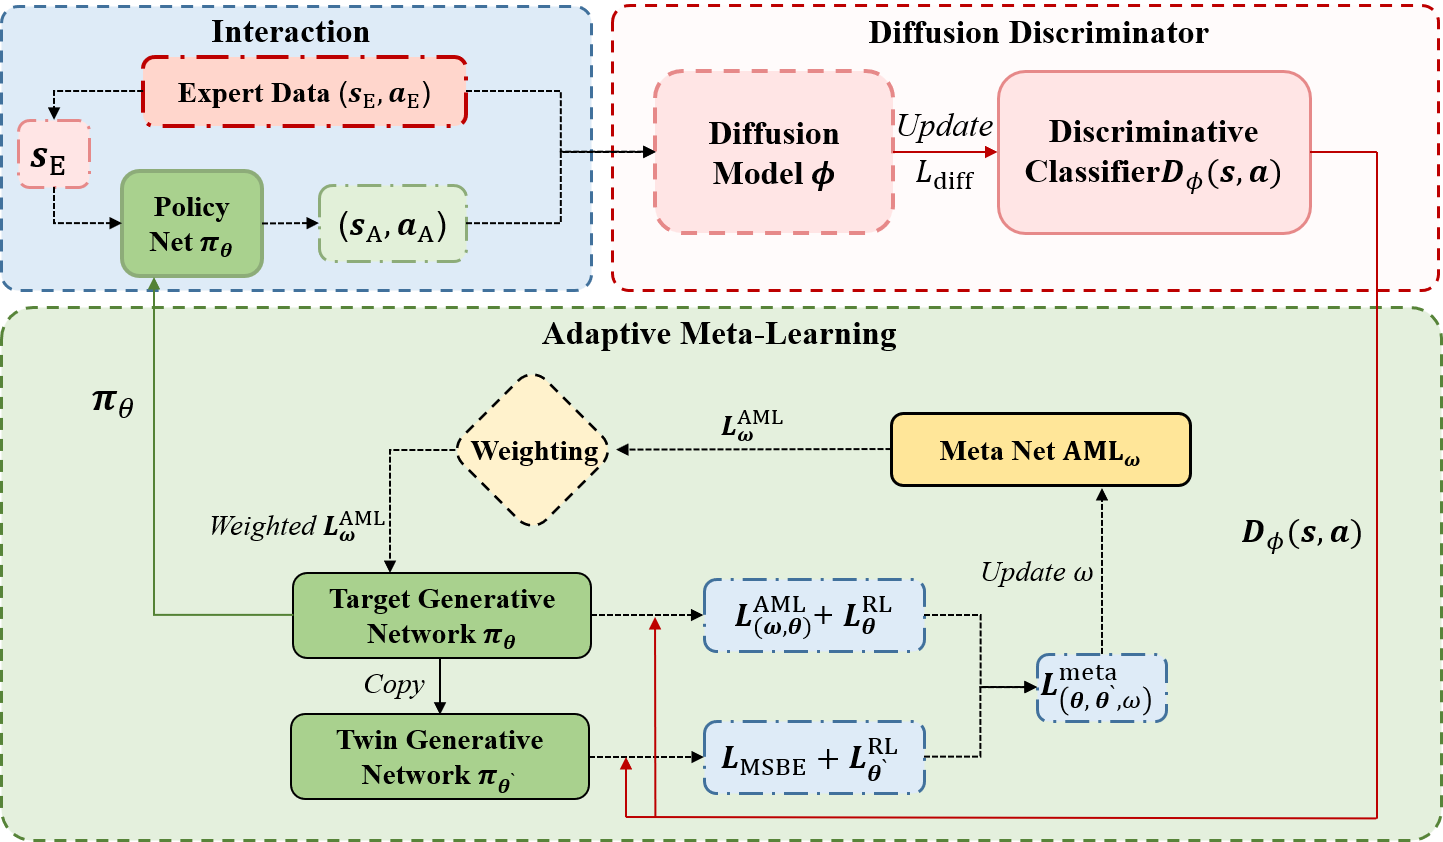
\includegraphics[width=5.5in]{AMLN.png}
\caption{The structural diagram of AMAIL consists of three parts: interaction, diffusion discriminator, and adaptive meta-generator. Solid lines represent the parameter transmission related to network updates, while dashed lines indicate the input and output of the actual data involved in the updates. When updating the generator, the reward used comes from the normalized reward generated by the discriminator during the interaction update, which will override the environment reward in the rollout.}
\label{fig_1}
\end{figure*}
When updating the target strategy network, the target generation network $\pi_{\theta}$ first makes a copy to generate a temporary twin generation network $\pi_{\theta'}$. These networks are connected as the lower-level network and the upper-level meta-network through parameter differentiation during network updates. The lower-level network uses the trajectories and rewards collected during the interaction process for backpropagation to enhance learning. During the reinforcement learning process, we introduce gradient losses from AML and IL to assist learning. After updating the two networks respectively, there are performance differences between the two networks. What the upper-level meta-network needs to learn is the inherent trend that the strategy learned by RL + AML is superior to that learned by RL + IL. This trend can be quantitatively represented by the difference in the objective functions of the two networks.

The basic update algorithm of the lower-level network is PPO update. The algorithm collects information during the interaction with the environment and stores it in rollouts. During the update process, the data in rollouts is used to calculate the discounted return and advantage function for each time step, and then enters multiple rounds of iterations. In the multiple rounds of iterations, the training process of each batch is divided into four stages. First, the target generation network is cloned, and at the same time, its parameters are ensured to be leaf nodes, which can be updated independently. Then, the RL and IL hybrid update of the twin generation network is carried out to calculate the new log probability and state value of the network's generated actions, and then subtract the log probability of the actions sampled from the old policy to obtain the probability ratio. The policy loss objective function is as follows:
\begin{flalign}
  \label{Agent_loss}
  &L^{\prime}_{\text{CLIP}}=E[\text{min}(\varDelta_{\ell(\theta)} \cdot A_{\pi}(s,a), \nonumber&\\
  &\quad \quad \quad\quad \quad\quad \quad\text{clip}(\varDelta_{\ell(\theta)},1-\epsilon ,1+\epsilon )\cdot A_{\pi}(s,a))]&
\end{flalign}
Here, $\varDelta_{\ell(\theta)}$ represents the difference in logarithmic probabilities between the new and old strategies, and $A_{\pi}(s,a)$ is the advantage function obtained by calculating the discounted return at each time step.

The value function part adopts the clipped mean square error to ensure that the update of the critic is not too large. The loss function of the value function is as follows:
\begin{equation}
\label{Value_loss}
V^{\prime}_{\text{loss}}=0.5\cdot \text{max}[(V^{\prime}-r)^2,(V^{\prime}_{\text{clip}}-r)^2]
\end{equation}
At the same time, IL is introduced. Here, behavior cloning is used, and expert data from the same batch as reinforcement learning is employed. The final optimized total loss function is:
\begin{equation}
\label{tmp_loss}
L^{\prime} = L^{\prime}_{a} + c_{\text{v}} \cdot V^{\prime}_{\text{loss}} + c_{\text{bc}} \cdot L^{\text{BC}} - c_{\text{ent}} \cdot \mathbb{E}[H^{\prime}(x)]
\end{equation}
Among them, $c_\text{v}$, $c_{\text{bc}}$, and $c_{\text{ent}}$ are coefficients. This objective is used to update the twin generative network independently. After optimization, its loss value will serve as the reference benchmark for the subsequent AMLN update.

Then, using RL and AML to update the target generative network, in addition to the standard PPO loss, the AML loss is introduced. The AML part uses the target generative network to be updated to generate actions, and these actions are concatenated and passed into the AML network to obtain the initial meta-loss for the target generative network. Then, the discriminator estimates the learning weight $W$ of the AML loss. Thus, the loss of our AML is defined as
\begin{equation}
  L^{\text{AML}}_{(\omega,\theta)}=\mathbb{E}[f_{\text{AML}}\cdot W]
\end{equation}
The optimization objective function of the target generation network is:
\begin{equation}
\label{actor_loss}
  L = L_{a} + c_{\text{v}} \cdot V_{\text{loss}} + L^{\text{AML}}_{(\omega,\theta)} - c_{\text{ent}} \cdot \mathbb{E}[H(x)]
\end{equation}

During the update process of the lower-level network, AMLN will take the state-action pair $(s^d, a^d)$ and the actor's action $a = \pi_\theta(s^d)$ as the input. To update the upper-level network AMLN, the meta-loss must contain differentiable AMLN parameters $\omega$, as shown in the figure. The upper-level network and the lower-level network establish a connection through differentiable parameters. The lower-level network quantitatively represents the superiority of the strategy learned by the upper-level AMLN during the RL+AMLN learning process compared to the strategy learned using RL+IL:
\begin{equation}
\label{AMLN_loss}
L^{\text{meta}}_{(\theta,\theta^{\prime},\omega)}= \text{tanh}(L_{\pi_{\theta^{\prime}}}-L_{\pi_{\theta}})
\end{equation}
Here, $L_{\pi_{\theta^{\prime}}}$ represents the loss of the twin network policy (including BC), while $L_{\pi_{\theta}}$ represents the loss of the target generation network (including AML).

Then, by taking the negative of this equation and using backpropagation, AMLN is updated to improve the performance of the policy, making it superior to the pure BC policy.
\begin{algorithm}[H]
\caption{algorithm of AMLN}\label{alg:AML}
\begin{algorithmic}[1]
\REQUIRE Policy network $\pi_\theta$, Discriminator $D_\phi$, AMAIL network $G_\omega$, Expert demonstrations $\mathcal{D}_E$, Rollouts $\mathcal{R}$
\ENSURE Optimized policy network $\pi_{\theta^\star}$, Learned AML network $G_{\omega^\star}$
\STATE \textbf{for} $epoch = 1,2,...,N_{epochs}$ \textbf{do}
\STATE \hspace{0.5cm}Sample mini-batches $\mathcal{B} \sim \mathcal{R} $
\STATE \hspace{0.5cm}\textbf{for} each mini-batch $\mathcal{B}$ \textbf{do}
\STATE \hspace{1cm}Clone policy: $\theta^{\prime}\leftarrow \theta$
\STATE \hspace{1cm}Calculate PPO surrogate loss via Eq. \eqref{Agent_loss}
\STATE \hspace{1cm}Calculate clipped value loss via Eq. \eqref{Value_loss}
\STATE \hspace{1cm}Sample expert data $(s_E,a_E) \sim \mathcal{D}_E$
\STATE \hspace{1cm}Calculate behavior loss $L^{\text{BC}}=\lVert \pi_{\theta^{\prime}}(s_E)-a_E \rVert_2^2$
\STATE \hspace{1cm}Update the twin network using loss $L^{\prime}$ via Eq. \eqref{tmp_loss}
\STATE \hspace{1cm}Evaluate PPO loss using $\pi_{\theta}$
\STATE \hspace{1cm}Generate policy actions $a_\theta=\pi_\theta(s_E)$
\STATE \hspace{1cm}Calculate AMLN output $f_{AML}([a_\theta,s_E,a_E])$
\STATE \hspace{1cm}Calculate total policy loss via Eq. \eqref{actor_loss}
\STATE \hspace{1cm}Update policy network $\theta$ using loss $L$
\STATE \hspace{1cm}Update AMLN via Eq. \eqref{AMLN_loss}
\STATE \hspace{0.5cm}\textbf{end for}
\STATE \textbf{end for}
\end{algorithmic}
\label{alg1}
\end{algorithm}
\subsection{Adaptive Learning Weights}
In the model architecture, the experience provided by the upper-level AMLN is actually a more superior form of imitation learning. It aims to learn the policy $\pi_\theta\left(a\mid s\right)$ through the data of experts (demonstrators) to imitate the expert policy $\pi_E\left(a\mid s\right)$. This approach also inherits the drawbacks of imitation learning, namely, the model's performance is highly dependent on expert demonstrations, and it is vulnerable to distribution drift. Under noisy conditions, small errors in the model can accumulate exponentially, weakening the learning speed and effectiveness of the model. For adversarial learning, teaching noise can cause the discriminator to learn a blurred boundary, thereby generating a regularization effect. However, when the noise is too large, the discriminator cannot distinguish the ``correct behavioral patterns'', and the learning direction will drift. Usually, we use confidence to weight the learning, making the weight of samples with high noise small to reduce their impact.

Regarding the calculation of weights, we use the diffusion loss generated during the diffusion of the discriminator to quantify the similarity of the state space probability distribution between expert data and generated data.

In reinforcement learning, we adjust the policy by having the model explore the environment and obtain feedback to learn the optimal policy. During the learning process, we typically calculate the discounted rewards the model receives during interactions based on the Markov decision process:

\begin{equation}
\eta (\pi)=\mathbb{E}_{\pi} \left[ \sum_{t=0}^{T} \gamma^t r(s_t,a_t) \right]
\end{equation}

Then we can use $\eta\left(\widetilde{\pi}\right) - \eta\left(\pi\right)$ to measure the performance superiority or inferiority between the two strategies $\widetilde{\pi}$ and $\pi$. However, sampling from strategy $\pi$ is rather difficult. We can approximate it by sampling from $\widetilde{\pi}$:

\begin{equation}
  L^{d_{\pi}}(\widetilde{\pi})=\sum_{s} d_{\pi}(s) \sum_{a} \widetilde{\pi}(a|s) A_{\pi}(s,a)
\end{equation}

Here, $d_{\pi(s)}=\mathbb{E}[\sum_{t=0}^{T} \gamma^t \mathbf{1}(s_t=s)]$ represents the state visitation distribution of the strategy $\pi$, and $\mathbf{1}$ is the indicator function.
In order for the strategy we train to outperform the original strategy, we need to maximize $L^{d_\pi}\left(\widetilde{\pi}\right)$, while we also need to ensure that the strategy we train does not deviate too much from the target strategy we are learning. We describe our requirements using the f-divergence constraint problem and obtain the expression of another strategy using the Lagrange multiplier method:

\begin{align}
\max_{\widetilde{\pi}}\quad & L^{d_{\pi}}(\widetilde{\pi}) - \beta D_{f}\!\big(\rho_{\tilde{\pi}}\|\rho_{\pi}\big) \\
	\text{s.t.}\quad & \sum_{a}\widetilde{\pi}(a\mid s)=1,\quad \widetilde{\pi}(a\mid s)\in[0,1] \notag
\end{align}

Here, $\beta$ serves as a hyperparameter to balance the reliance of our learning strategy on the original expert strategy. Solving the system of equations yields:


\begin{gather}
\widetilde{\pi}(a \mid s)=\pi(a \mid s) f_{*}^{\prime}\left((1 / \beta)\left(A_{\pi}(s, a)+C(s)\right)\right)\notag \\
f^{*}(p)=p u-f(u)\notag \\
\widetilde{\pi}(a \mid s)=\pi(a \mid s) \exp \left((1 / \beta)\left(A_{\pi}(s, a)+C(s)\right)\right)
\end{gather}

The work of Yunke Wang et al. verified that the $\widetilde{\pi} $ calculated by this method is superior to $\pi$. This equation can be expressed in the form of an action space distribution:

\begin{equation}
\rho_{\widetilde{\pi}}(s, a)=\rho_{\pi}(s, a) \exp \left((1 / \beta)A_{\pi}(s, a)\right)
\end{equation}

Analogous to WGAIL, the weight $\omega$ satisfies

\begin{equation}
  \rho_{\widetilde{\pi}}(s, a)= \omega(s, a)\rho_{\pi}(s, a) 
\end{equation}

This means that $\omega \propto A_\pi$.

Given the connection between $\omega$ and $A_\pi$, in our actual experiments, we approximated $\omega$ using $D$ and $\pi$ obtained through the diffusion discriminator. In the diffusion discriminator, $\mathcal{L}_{\text{diff}}$ was used to measure the direct similarity of the action transfer space. The label $c+$ indicated data that fitted the expert data, while the label $c-$ corresponded to the agent data. The values with a larger range were re-normalized by a fraction to be within the range of a binary classifier.

\begin{flalign}
D_{\phi}(s,a) &= \frac{e^{-\mathcal{L}_{\text{diff}}(s,a,c^+)}}{e^{-\mathcal{L}_{\text{diff}}(s,a,c^+)}+e^{-\mathcal{L}_{\text{diff}}(s,a,c^-)}} \notag\\
&= \sigma(\mathcal{L}_{\text{diff}}(s,a,c^-)-\mathcal{L}_{\text{diff}}(s,a,c^+)) \notag\\
&= \frac{\pi_{\theta}(a\mid s)}{\pi_{\theta}(a\mid s)+\omega(s,a)\pi(a \mid s)} \notag \\
&= \frac{\pi_\theta(a \mid s)}{\pi_\theta(a \mid s)+\omega(s , a)\text{exp}(A_\pi (s,a))}
\end{flalign}

In the work of Fu et al., it is demonstrated that $A(s,a)$ can be recovered by $\text{log}[\pi(a\mid s)]$. 

According to the above formula, we can obtain

\begin{equation}
D_{\psi }^{\ast }(s,a)=\frac{\pi_\theta(a \mid s)}{\pi_\theta(a \mid s)+\omega(s,a)^{(\beta+1)}}
\end{equation}

Ultimately, our weights can be expressed as:

\begin{equation}
  \omega(s,a)=[(1/D_\psi ^{\ast }(s,a)-1)\pi_\theta(a \mid s)]^{\frac{1}{\beta+1}}
\end{equation}

The weighted-adjusted AML loss can, to a certain extent, enhance the model's performance and can mitigate the accumulation of errors in class imitation learning caused by suboptimal expert data and environmental noise.

\section{Experiment}
\begin{figure*}[!t]
\centering

\subfloat[FETCHPUSH]{%
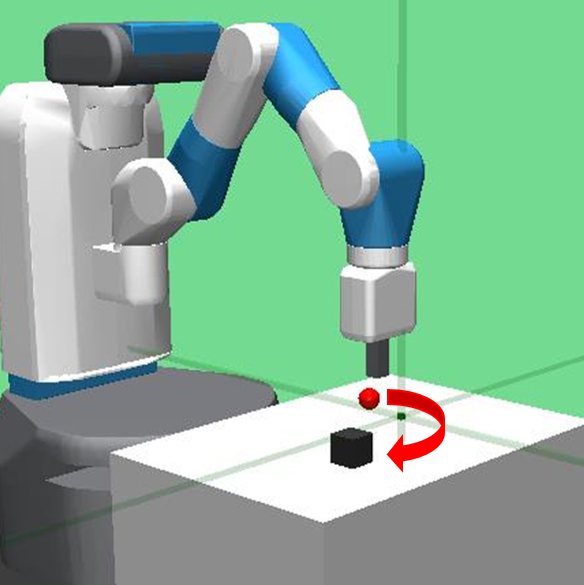
\includegraphics[width=0.19\textwidth]{pic1}%
\label{fig_first_case}}%
\hfill
\subfloat[FETCHPICK]{%
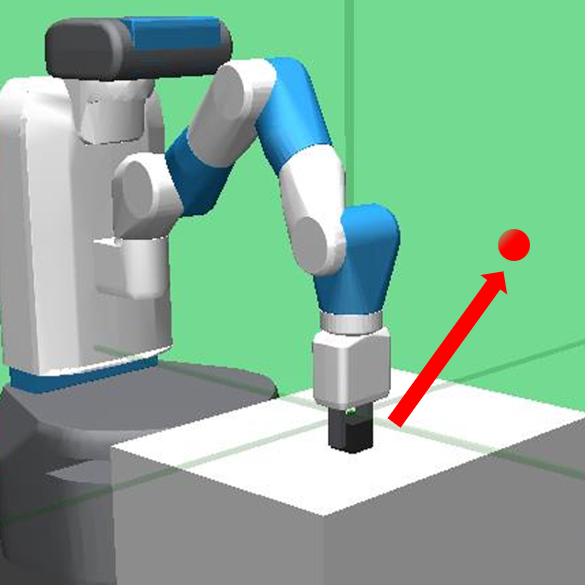
\includegraphics[width=0.19\textwidth]{pic2}%
\label{fig_second_case}}%
\hfill
\subfloat[ANTREACH]{%
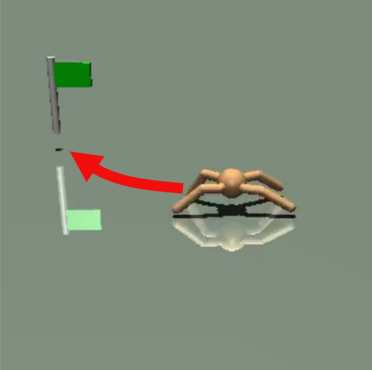
\includegraphics[width=0.19\textwidth]{pic3}%
\label{fig_third_case}}%
\hfill
\subfloat[HANDROTATE]{%
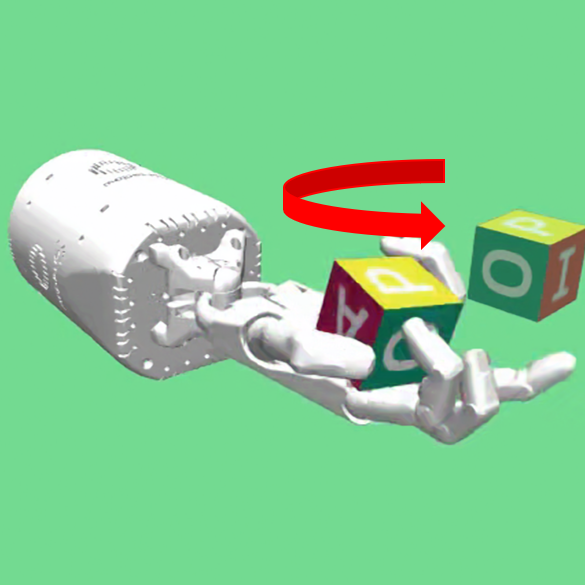
\includegraphics[width=0.19\textwidth]{pic4}%
\label{fig_fourth_case}}%
\hfill
\subfloat[MAZE]{%
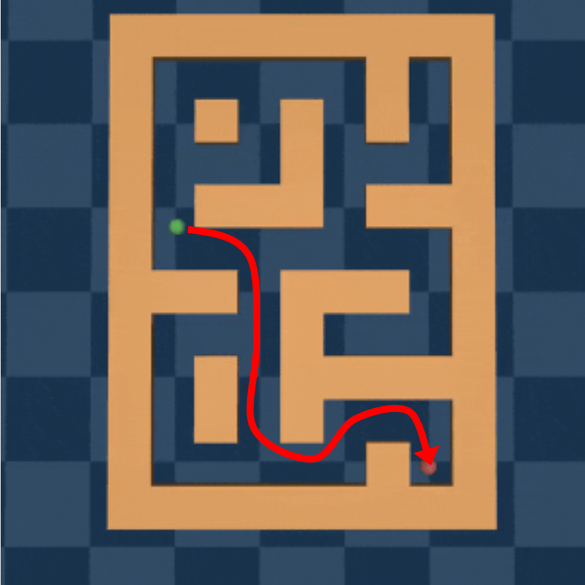
\includegraphics[width=0.19\textwidth]{pic5}%
\label{fig_fifth_case}}%

\caption{The experiments mainly consist of five goal-oriented tasks. (a) The robotic arm needs to push the object to the target point. (b) The robotic arm needs to pick up the object and move it to the target point. (c) The ant agent needs to move to the target point indicated by the flag. (d) The dexterous hand needs to rotate the cube in its hand to the target direction. (e) The agent needs to pass through the maze from the green starting point to reach the red target point.}
\label{fig_sim}
\end{figure*}
This section evaluates the performance and data utilization of the proposed AMAIL, demonstrating its superiority in a random environment, as well as its improvements in training efficiency and generalization compared to existing methods. The proposed framework has been extensively evaluated in various continuous control domains, including navigation, robotic arm operation, and motion, all of which were conducted on the MuJoCo platform. To prove the improved performance and expert sample utilization of the proposed method, the environment scenarios were expanded according to the settings described by Lee et al.
\subsection{Simulation setup}
This section presents the methods used to evaluate AMAIL in terms of its environment, tasks, and expert demonstrations.

\textbf{FETCHPUSH.} We evaluate our approach on the 7-DoF FetchPush task (Fig. 3a), where the robot pushes a black block to a target location marked by a red sphere. The 16-dimensional observation includes the gripper pose, object pose, gripper-object relative pose, and goal position, with randomized initial and goal states. We use demonstrations from Lee et al. with 20,311 transitions (664 trajectories), and inject noise into initial and goal positions during training to test robustness.

\textbf{FETCHPICK.} In the FetchPick task (Fig. 3b), the agent must grasp and lift a block to a specified target position in the air. The state space composition is identical to FetchPush. For this task, we utilize a dataset of 50,000 transitions generated by a hard-coded policy. Similar to FetchPush, we inject additional noise into the initial and target block positions during training to evaluate the model's robustness.

\textbf{ANTREACH.} We also evaluate our method on AntReach (Fig. 3c), a high-dimensional locomotion task where a quadruped ant robot must navigate to a randomly generated target. The goal is positioned along the perimeter of a 5-meter radius semicircle centered on the agent. The 132-dimensional state vector encodes the robot's joint angles, velocities, contact forces, and the goal position relative to the agent. We use an expert dataset from Lee et al. containing 1000 demonstrations. To test for generalization, random disturbances are injected into the environment during policy training.

\textbf{HANDROTATE.} Finally, we evaluate our approach on HandRotate (Fig. 3d), a challenging high-dimensional manipulation task. In this environment, a 24-DoF Shadow Dexterous Hand must perform in-hand rotation of a block to a specified target orientation. The task is characterized by its high-dimensional state space (68-D) and action space (20-D). The state includes joint angles, velocities, the object's pose, and the target rotation. We use an expert dataset of 515 trajectories (10,000 transitions) collected by Lee et al.

\textbf{MAZE.} We also test our method in the MAZE navigation task (Fig. 3e), introduced by Fu et al. In this environment, a point-mass agent must navigate from a randomly sampled start location to a fixed goal. The agent observes its position and velocity and outputs continuous actions representing its target velocity in the x and y directions. For this task, we use the expert dataset provided by Lee et al. , which includes 100 demonstrations (18,525 transitions).

To evaluate our proposed AMAIL method, we compared AMAIL with the following representative baselines:

\textbf{$\bullet$ Behavior Cloning (BC)} is a supervised learning approach that directly learns a mapping from states to actions using expert demonstrations. It serves as a fundamental baseline for imitation learning.

\textbf{$\bullet$ Diffusion Policy (DP)} view the target policy network that needs to be trained as a conditional diffusion model. This model generates actions through the conditional diffusion process using the state and randomly sampled noise.

\textbf{$\bullet$ Generative Adversarial Imitation Learning (GAIL)}  formulates imitation learning as a minimax game between a policy and a discriminator, aiming to match the occupancy distributions of expert and policy-generated trajectories.

\textbf{$\bullet$ Wasserstein Adversarial Imitation Learning (WAIL)} introduce the Wasserstein distance to improve the GAIL objective function, making the rewards during network training more smooth.

\textbf{$\bullet$ Diffusion Adversarial Imitation Learning (DiffAIL)} introduces the diffusion model into adversarial imitation learning (AIL). By incorporating the diffusion loss as part of the discriminator's learning objective, it enables the discriminator to more accurately learn the distribution of expert data, thereby enhancing its ability to capture complex action distributions.

\textbf{$\bullet$ Diffusion Rewards Adversarial Imitation Learning (DRAIL)} integrates the diffusion model into GAIL, describing the closeness between the current state and the target state, aiming to generate more robust and smooth reward signals to overcome the instability problem in GAIL training.




\begin{figure*}[!t]
\centering

\subfloat[FETCHPUSH]{%
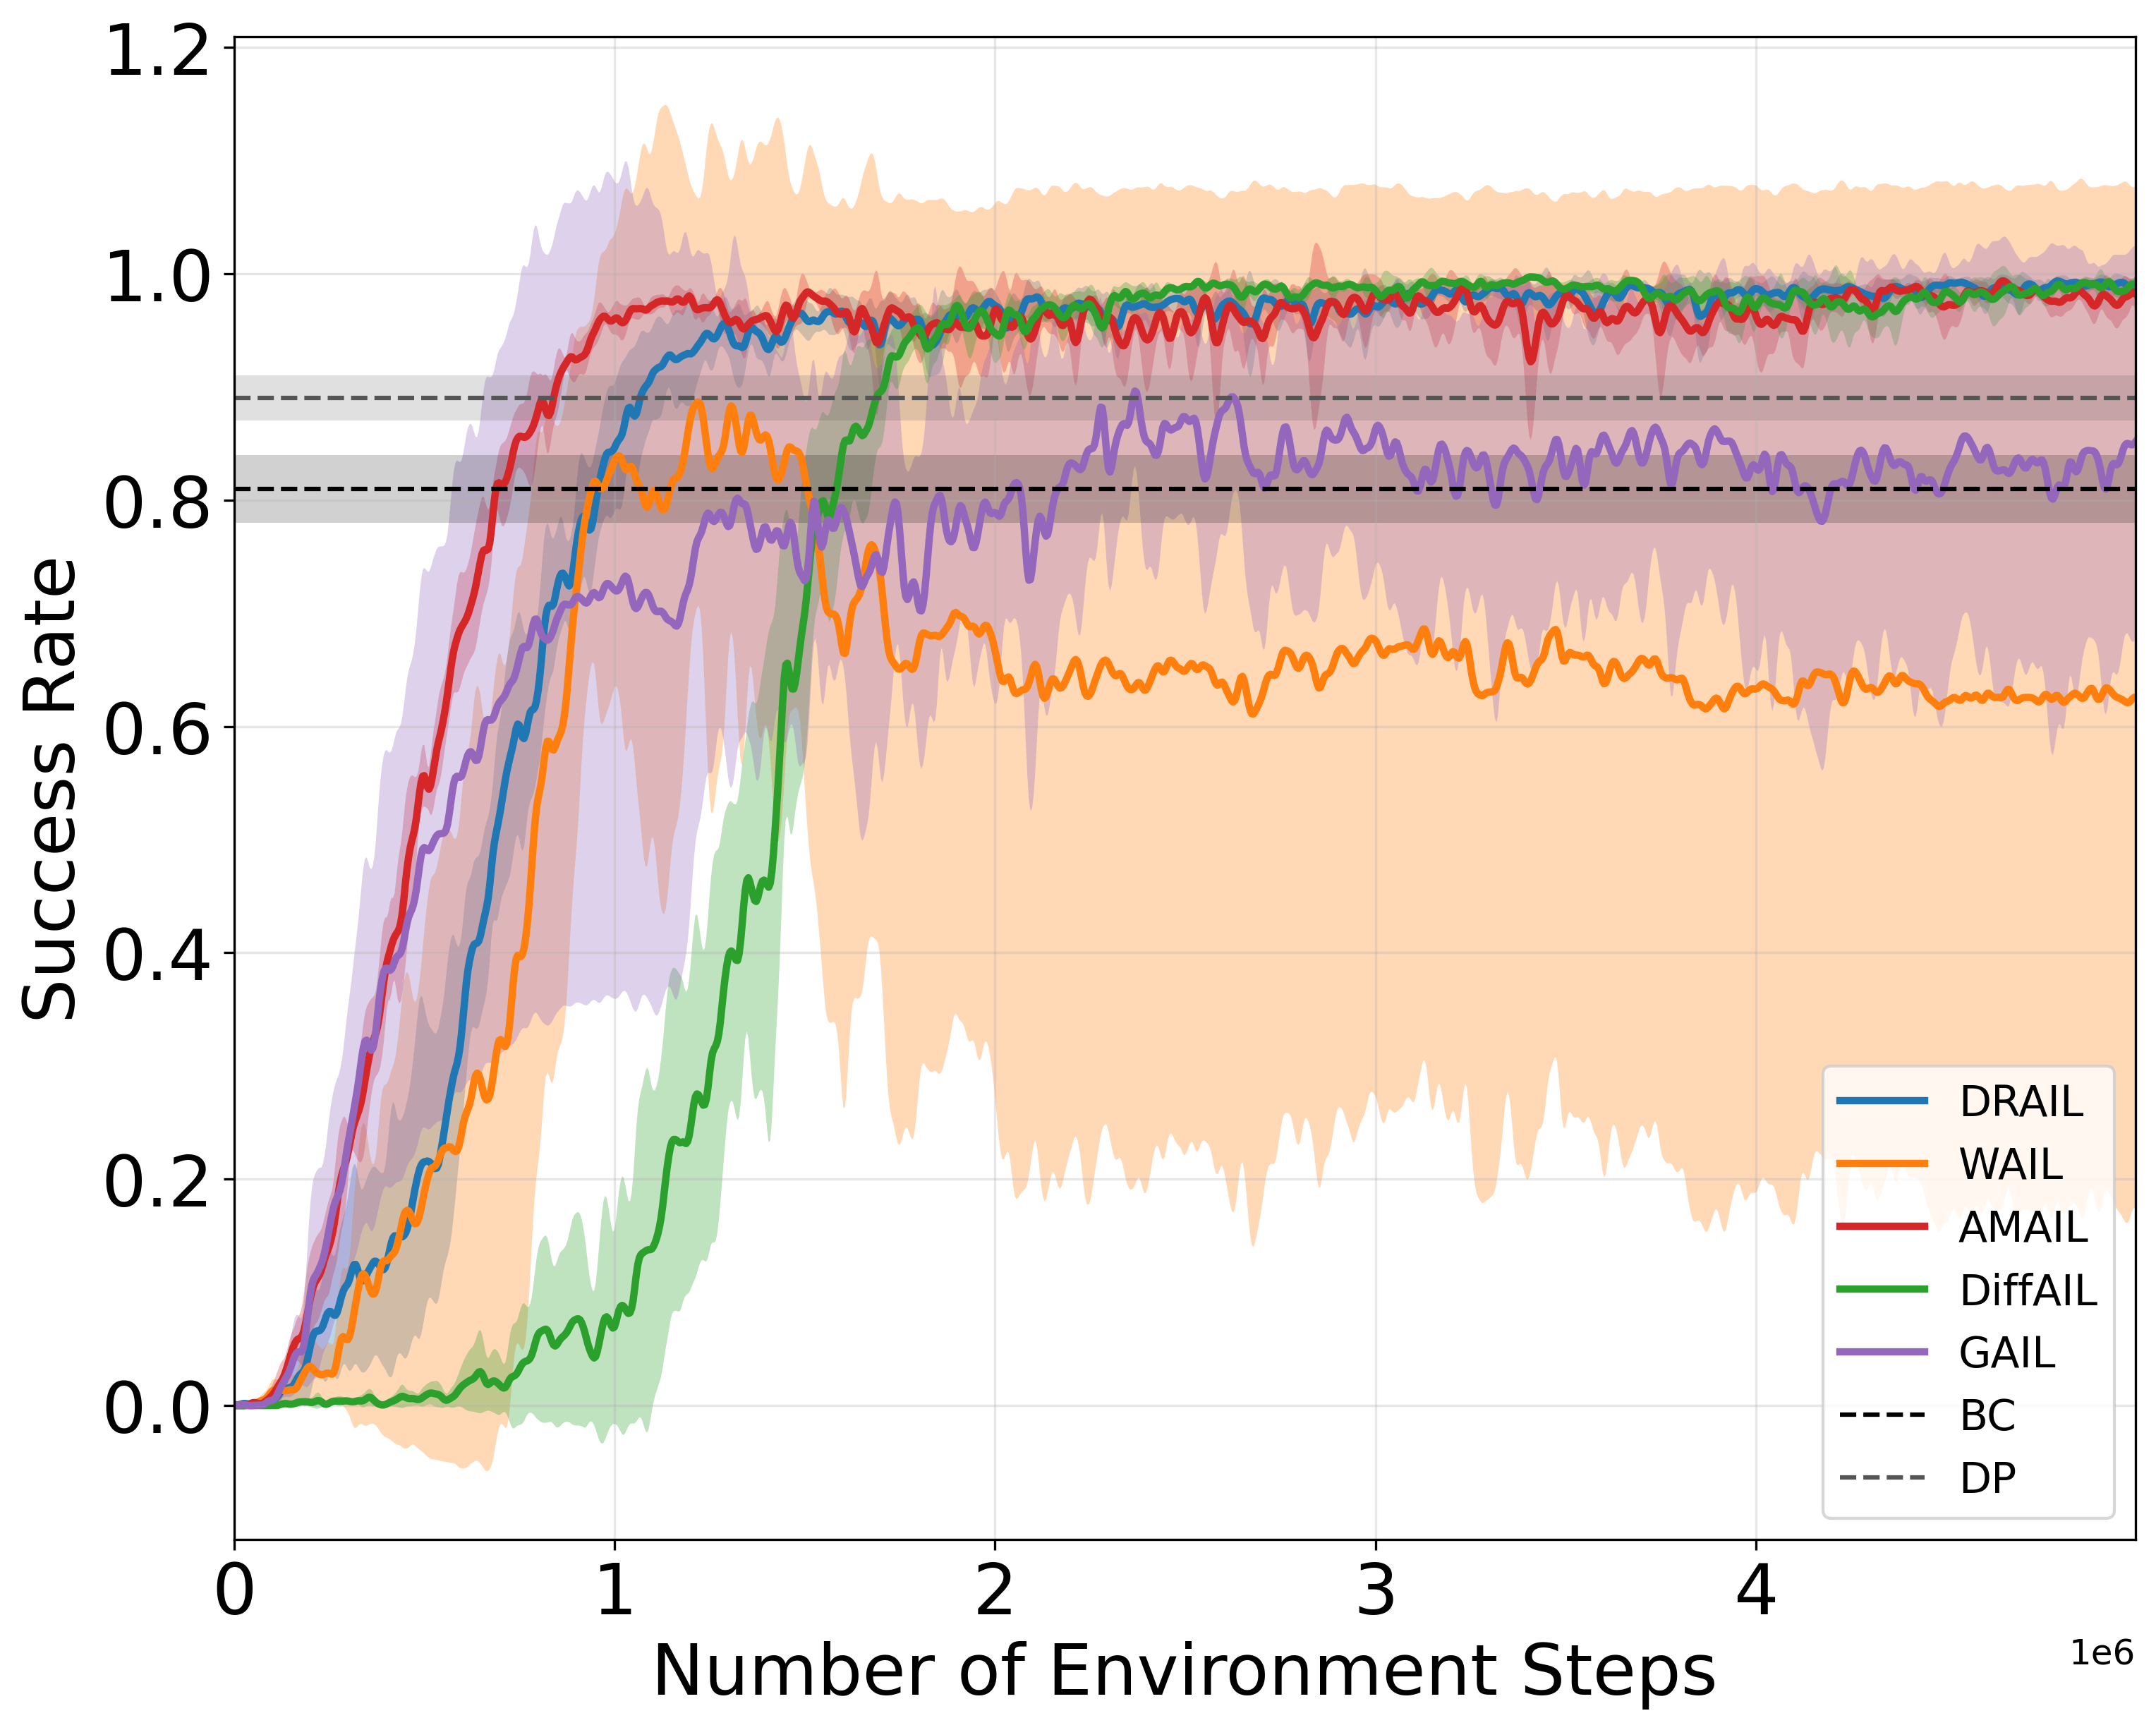
\includegraphics[width=0.33\textwidth]{fetchpush.png}%
\label{fetchpush}}%
\hfill
\subfloat[FETCHPICK]{%
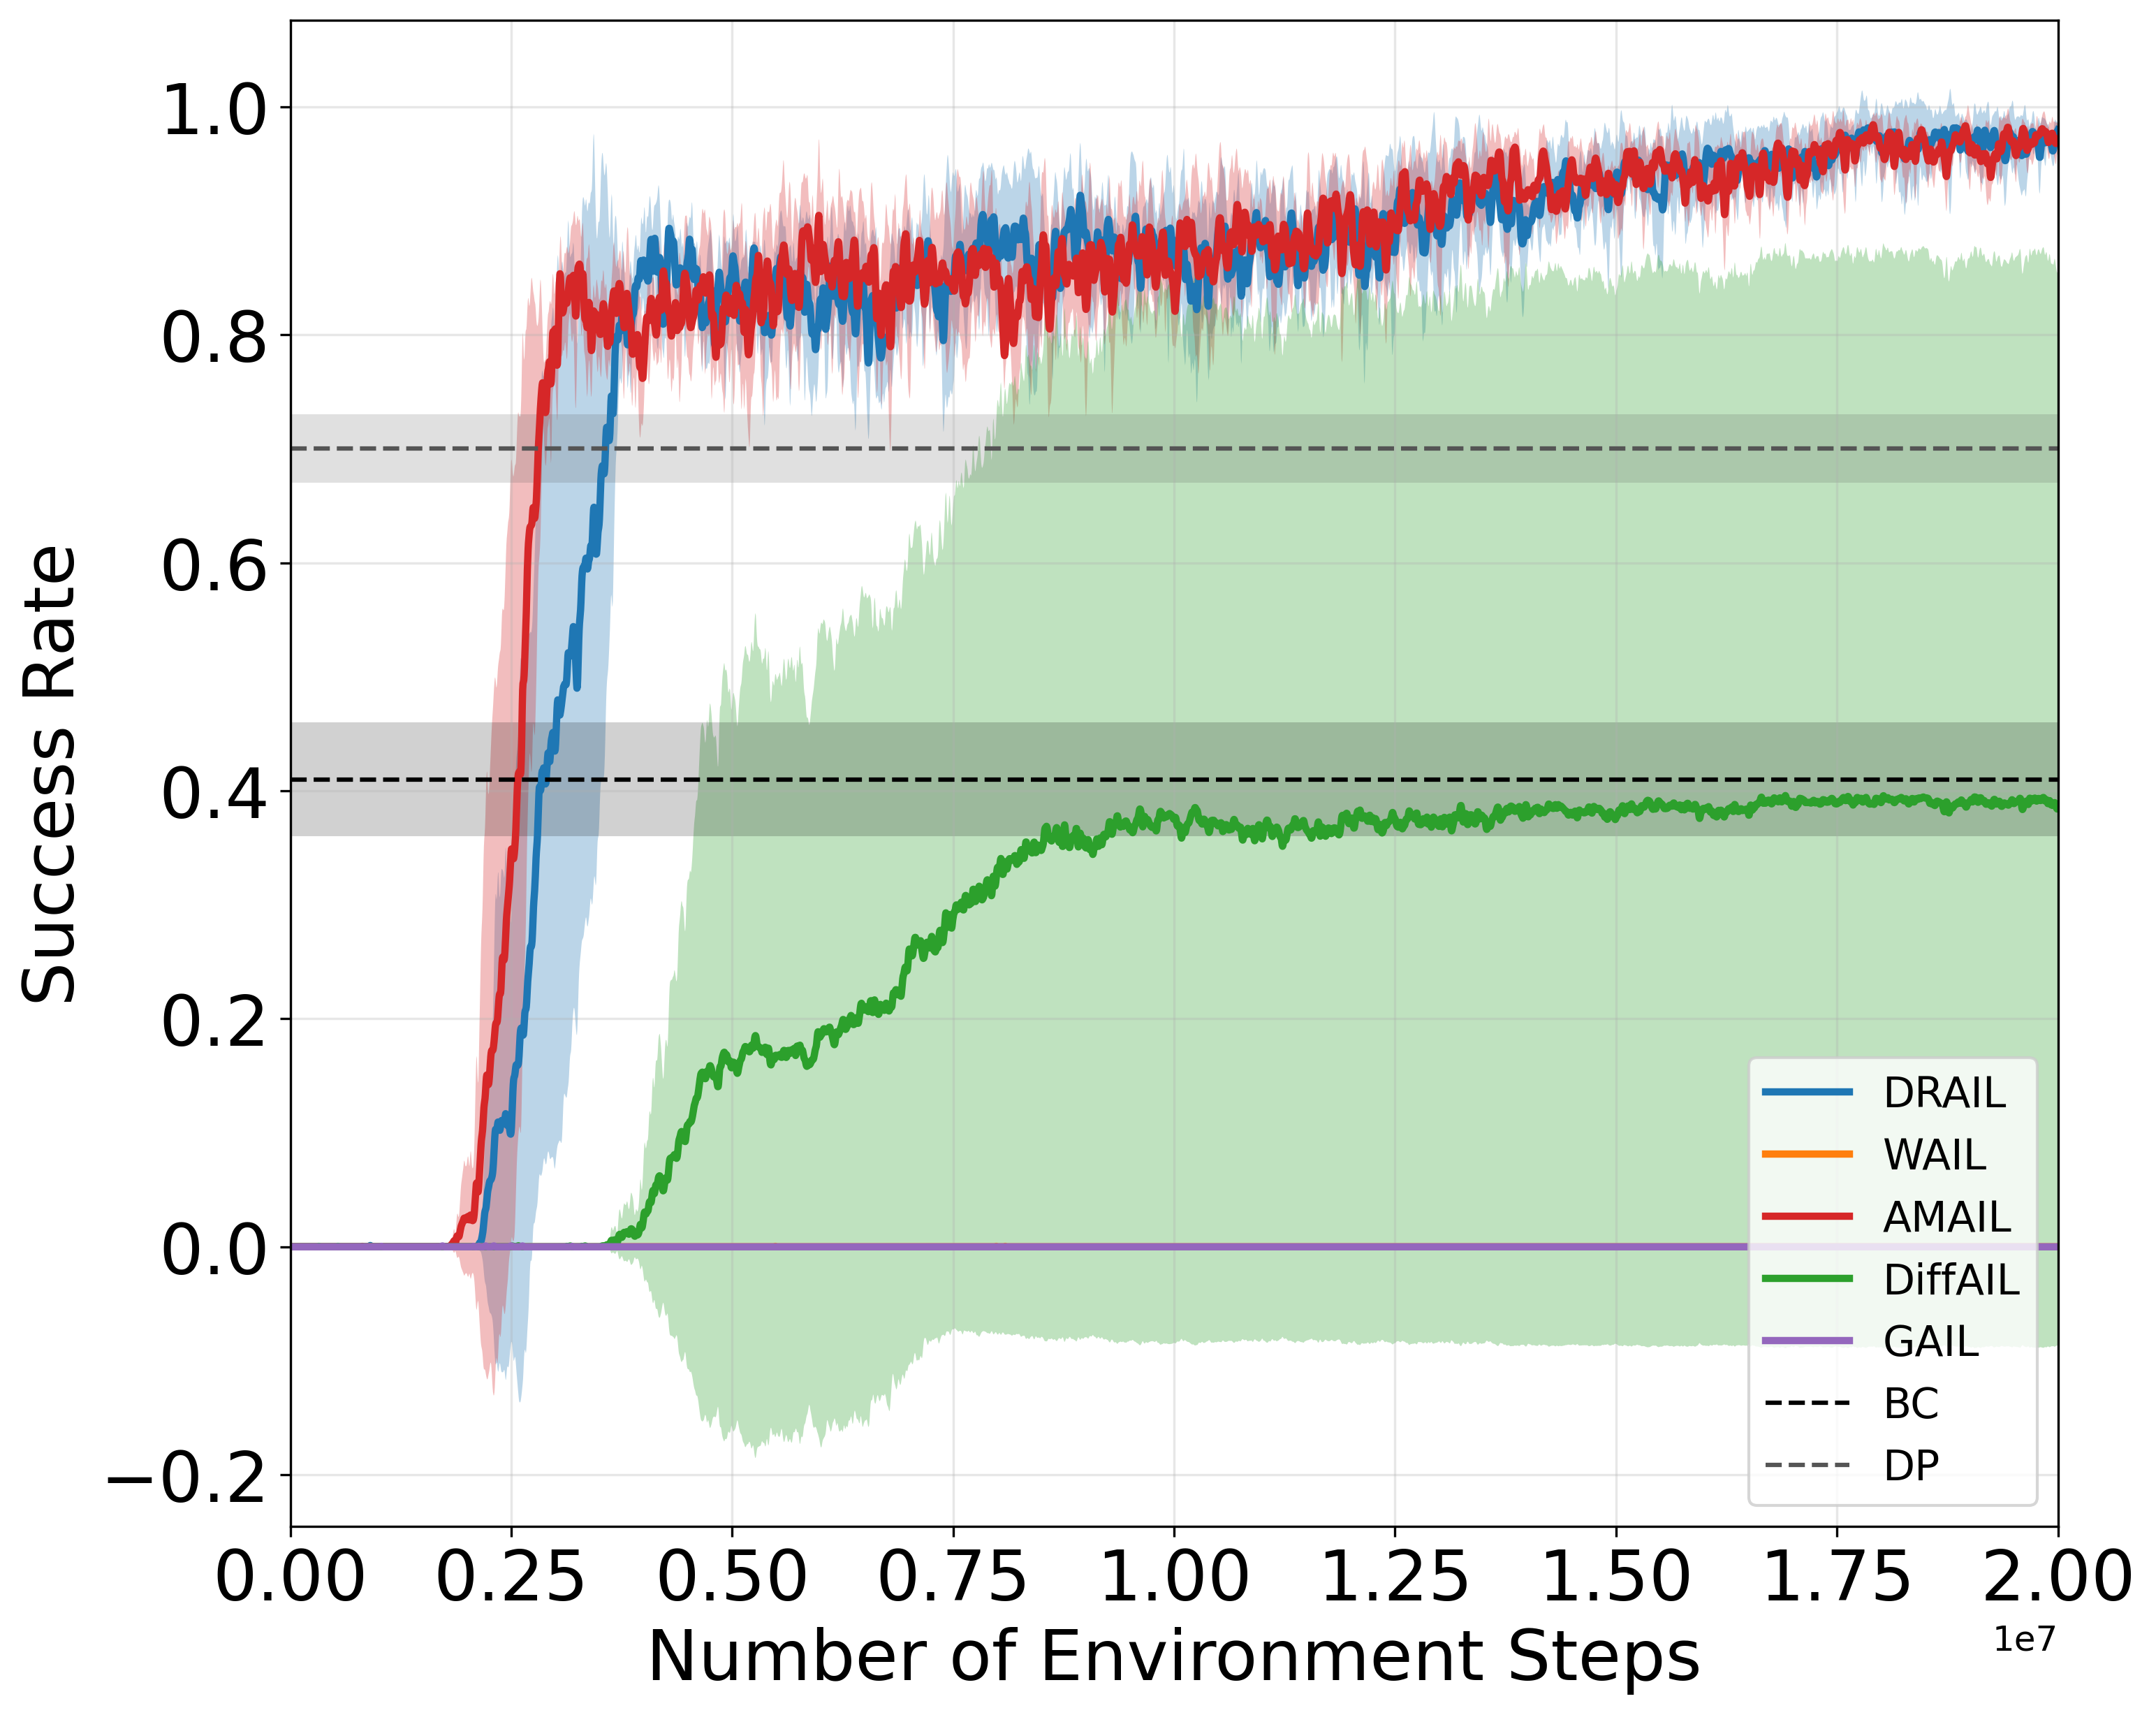
\includegraphics[width=0.33\textwidth]{fetchpick.png}%
\label{fetchpick}}%
\hfill
\subfloat[ANTREACH]{%
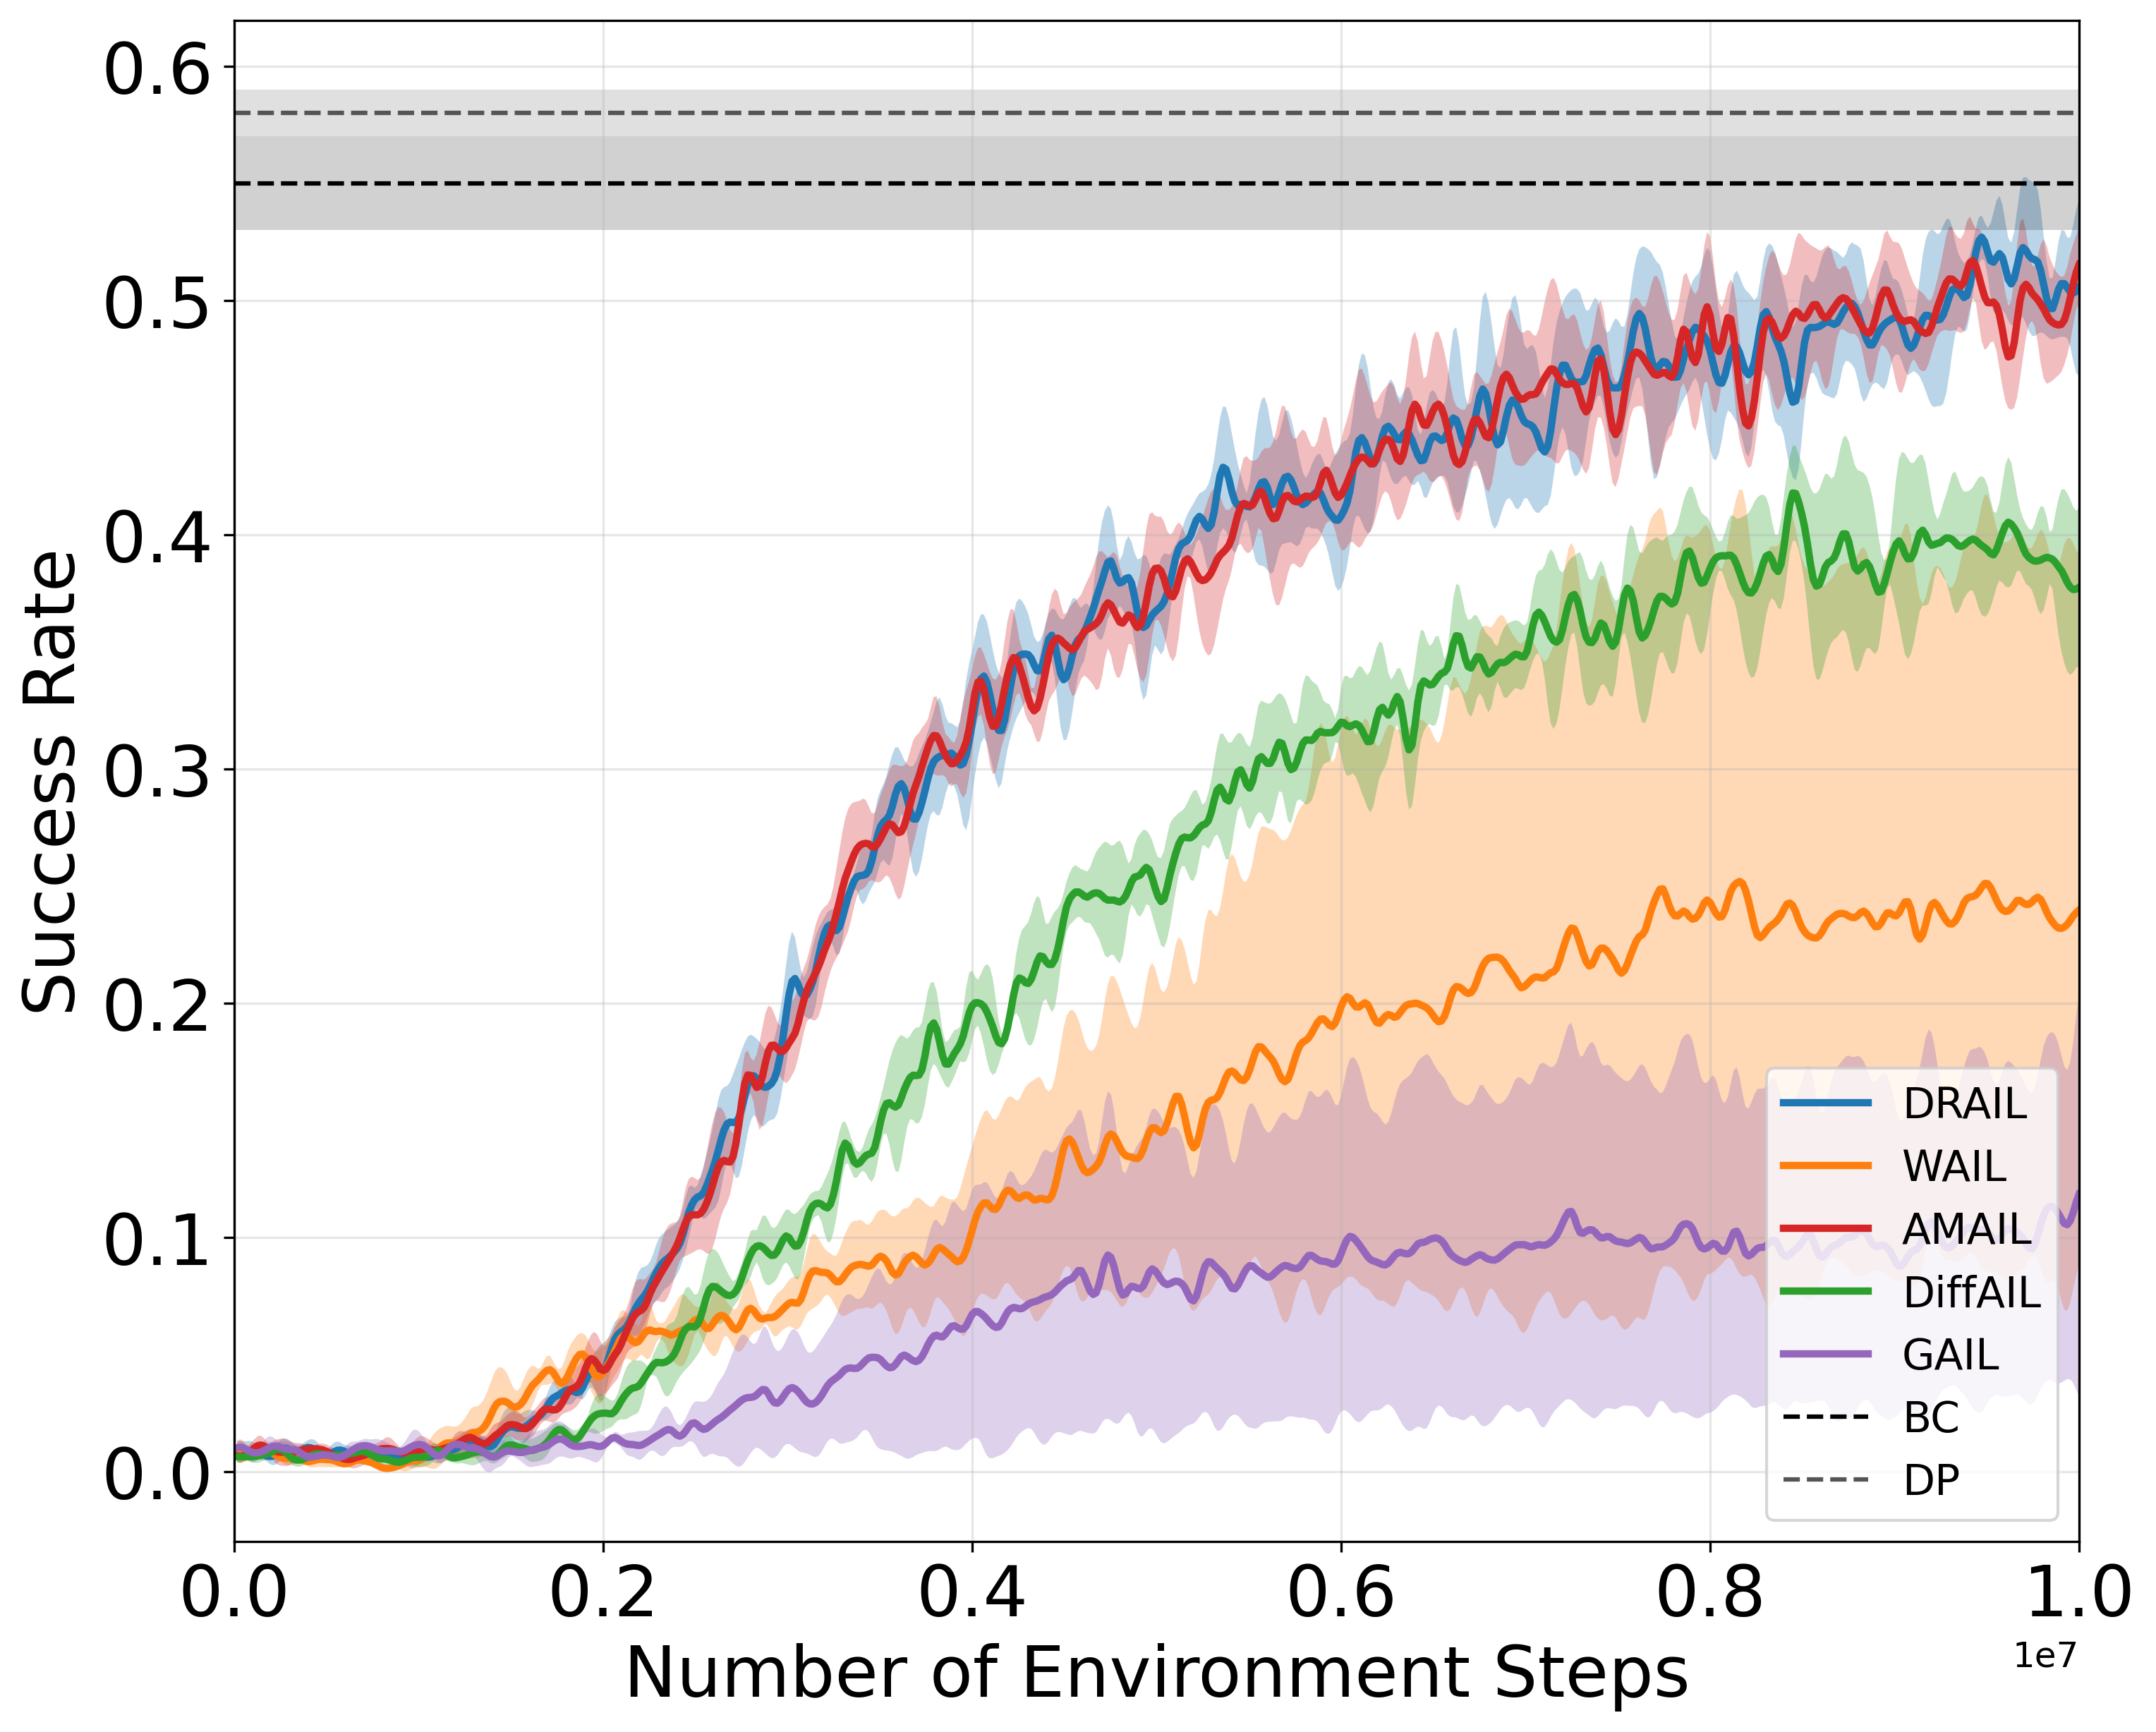
\includegraphics[width=0.33\textwidth]{Antgoal.png}%
\label{antreach}}%
\hfill
\subfloat[HANDROTATE]{%
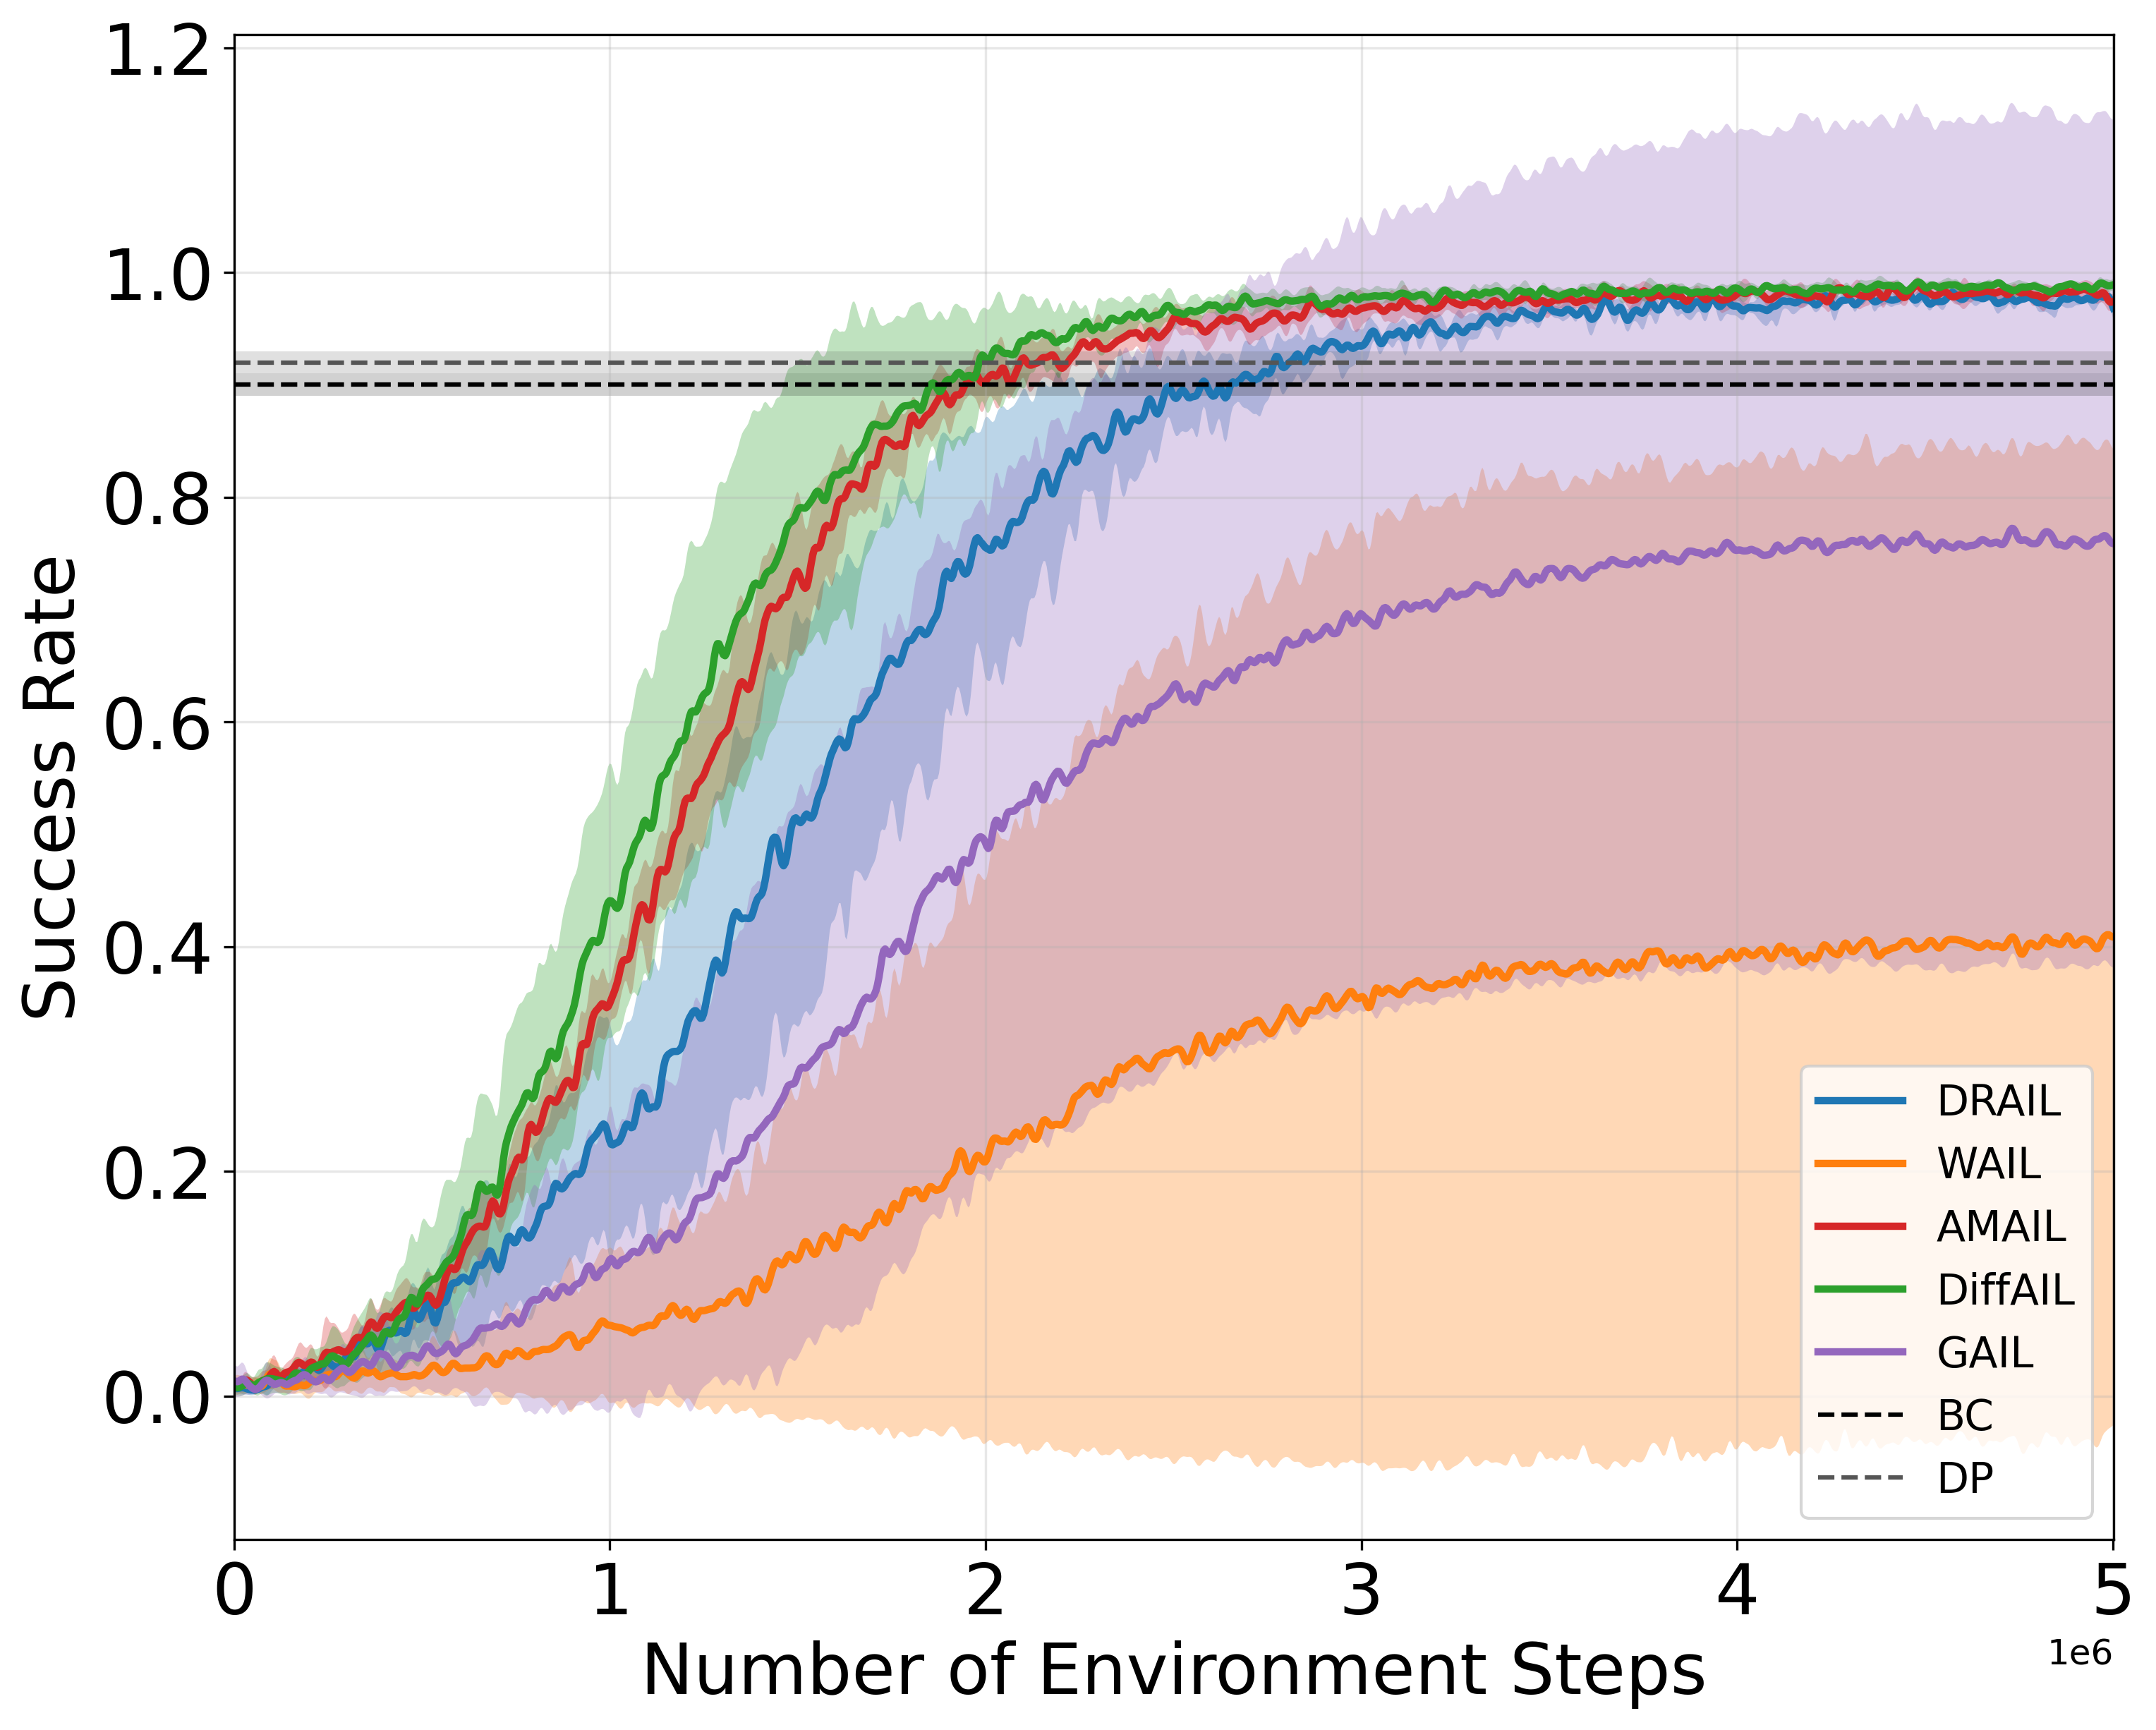
\includegraphics[width=0.33\textwidth]{Hand.png}%
\label{Hand}}%
\hspace{0.02\textwidth}
\subfloat[MAZE]{%
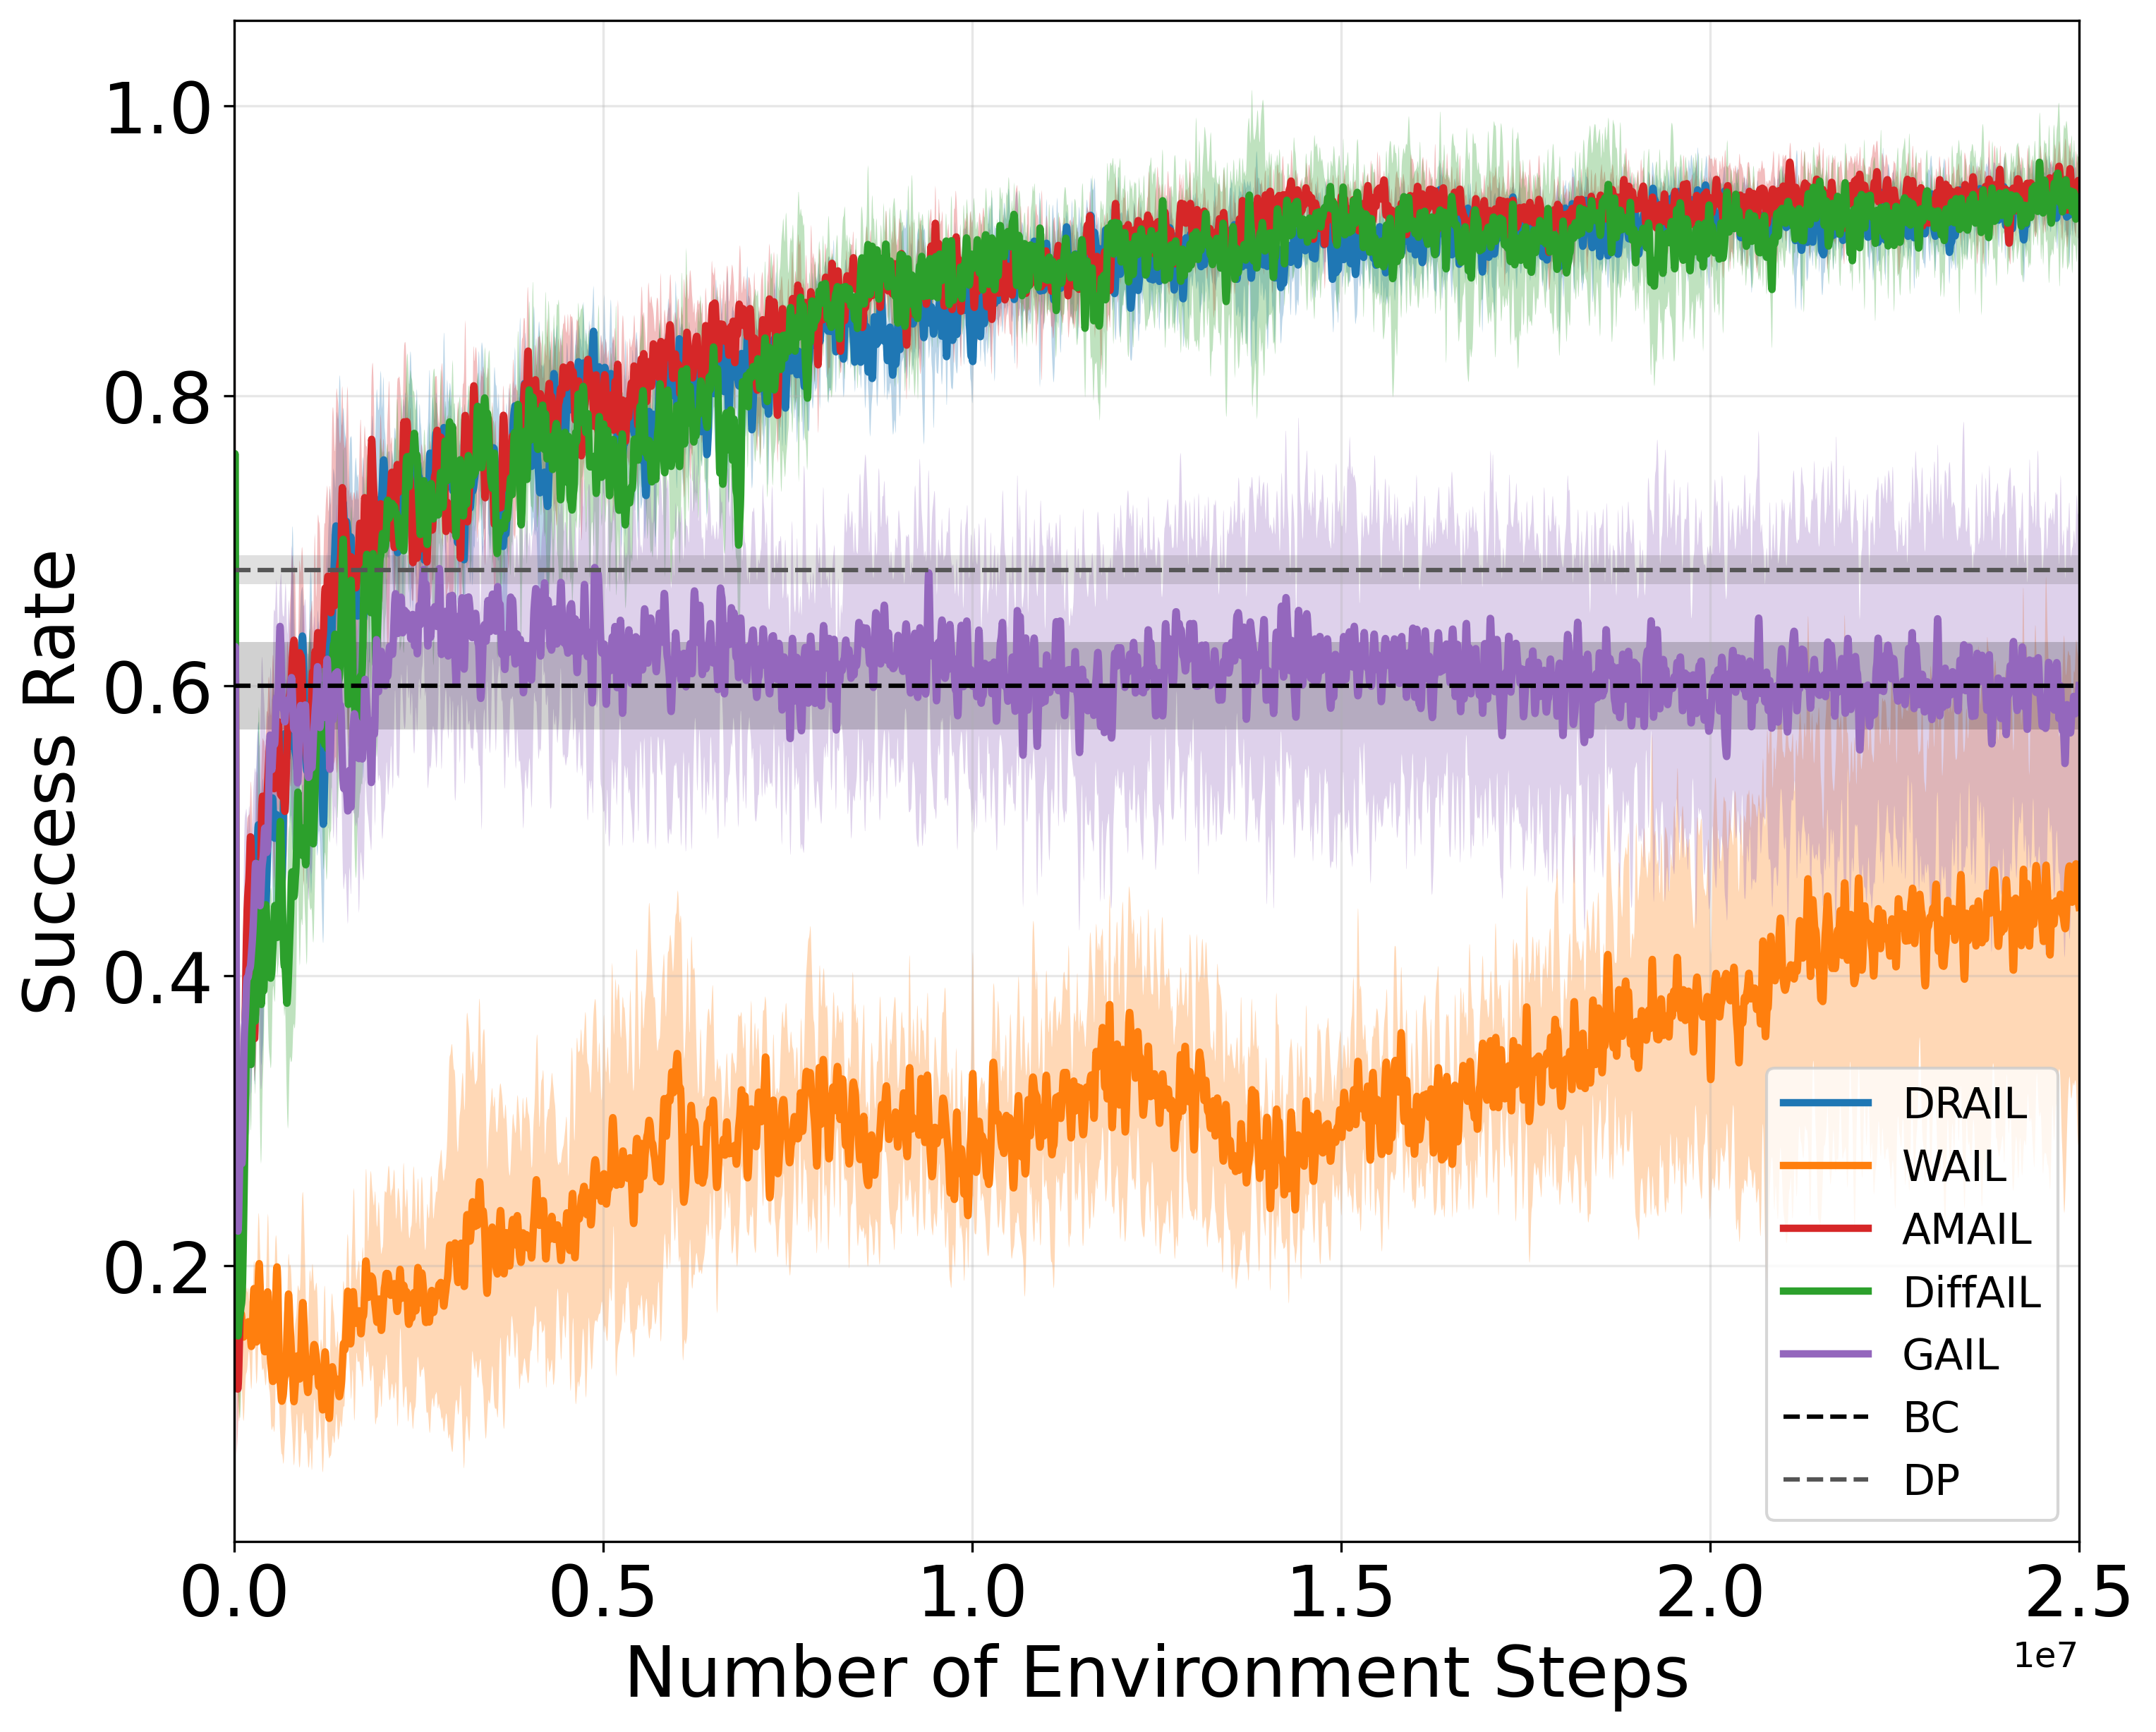
\includegraphics[width=0.33\textwidth]{Maze.png}%
\label{Maze}}%


\caption{\textbf{Learning efficiency}. Our method was compared with six other learning methods in five environments, and each environment was evaluated using five random seeds (the shaded area represents the pointwise standard deviation range of multiple experimental results, and the line represents the mean processing). Compared with other methods, our method is faster and more stable in all training stages and maintains excellent network performance.}
\label{fig_sim2}
\end{figure*}

To evaluate the performance of the learning methods, we trained all the methods using expert datasets in five environments. For each task, five different random seeds were used during training, and the standard deviation was plotted to reflect the stability of the model. Among them, BC and diffusion policy, as offline model-based learning algorithms, do not interact with the environment during the training process. Here, we set their success rate as a horizontal line.

Firstly, to evaluate the learning efficiency of each model under the expert setting standards, the complete expert dataset and the same noise setting (1x, the same as the expert data collection setting) were used for training in all tasks. Under the same conditions, our method achieved the performance of existing algorithms in all tasks and outperformed them in some tasks. AMAIL improves the utilization rate of expert data through meta-learning. It can quickly converge to expert-level performance in the FETCHPUSH, FETCHPICK, and HANDROTATE tasks, reflecting the effective guidance of the meta-learning network on the strategy network in learning the inherent logic of experts.

To further verify the improvement in data utilization achieved by AMAIL, we conducted experiments in the FTECHPUSH environment by reducing the amount of expert data. We reduced it to 2000, 5000, 10000, and the expert data (transformation). The results showed that AMAIL, by adopting a two-layer meta-learning architecture and using offline data for strategy guidance, improved the data utilization effect. The model, through learning the intrinsic logic of the expert data, provided additional guidance rewards. On one hand, this enhanced the model's exploration of high-value strategies; on the other hand, it reduced the confusion of low-value strategies. 

\begin{figure*}[!t]
\centering

\subfloat[10000 transitions]{%
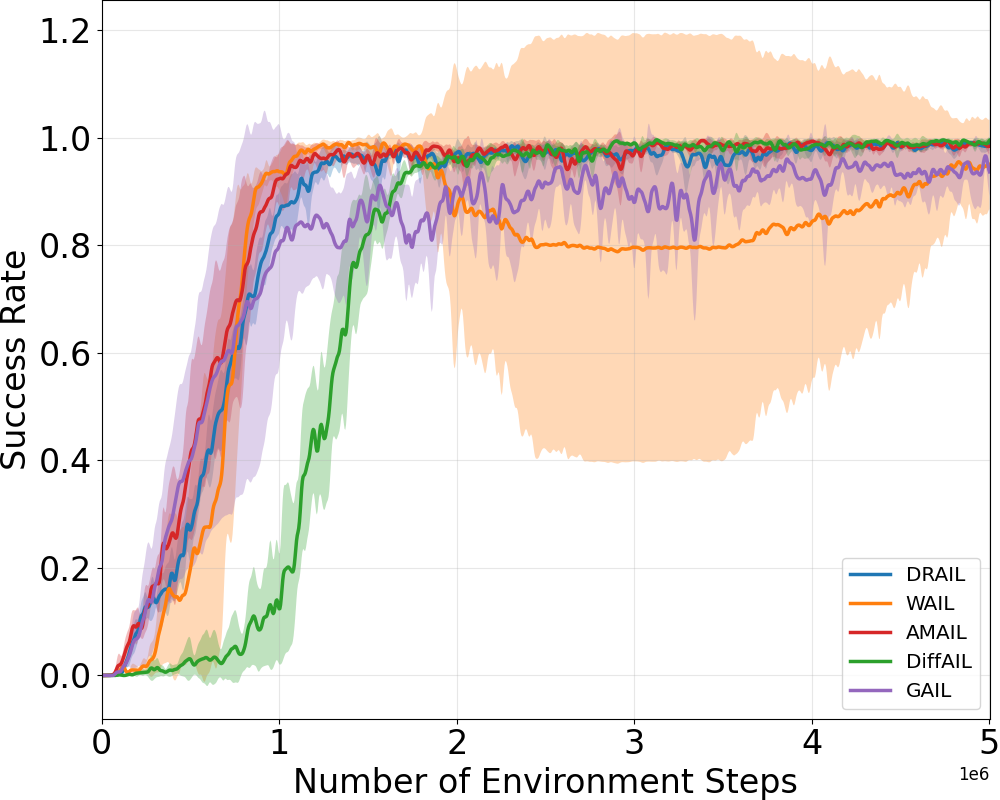
\includegraphics[width=0.33\textwidth]{10000.png}%
\label{FETCHPUSH 10000}}%
\hfill
\subfloat[5000 transitions]{%
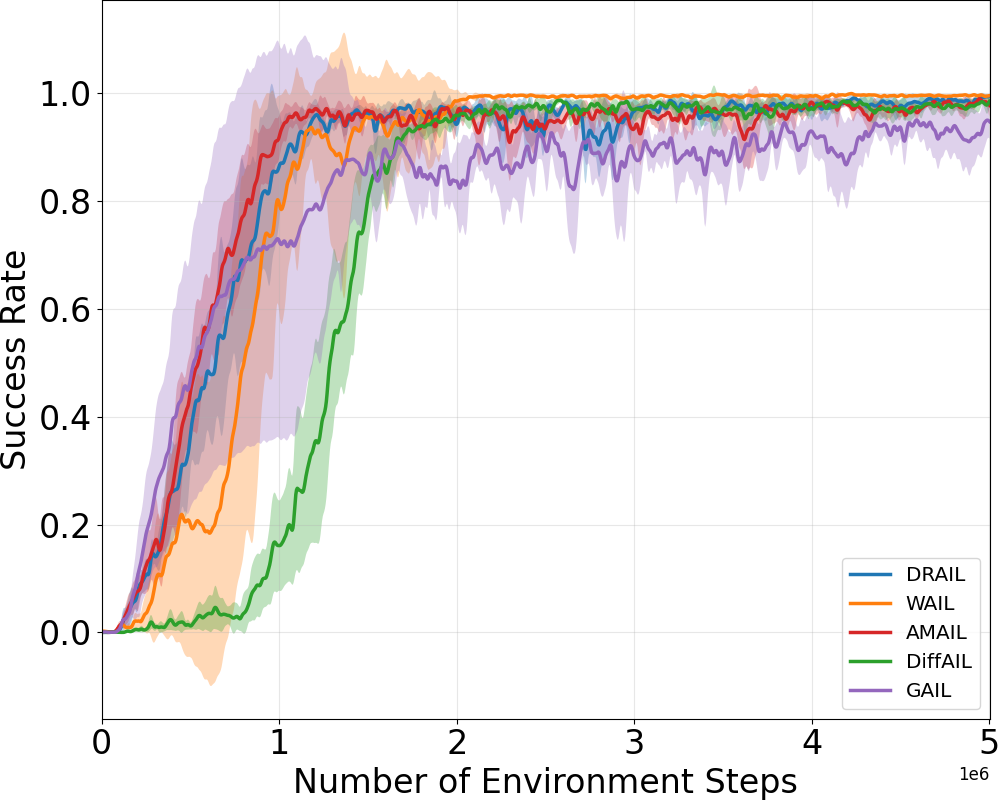
\includegraphics[width=0.33\textwidth]{5000.png}%
\label{FETCHPUSH 5000}}%
\hfill
\subfloat[2000 transitions]{%
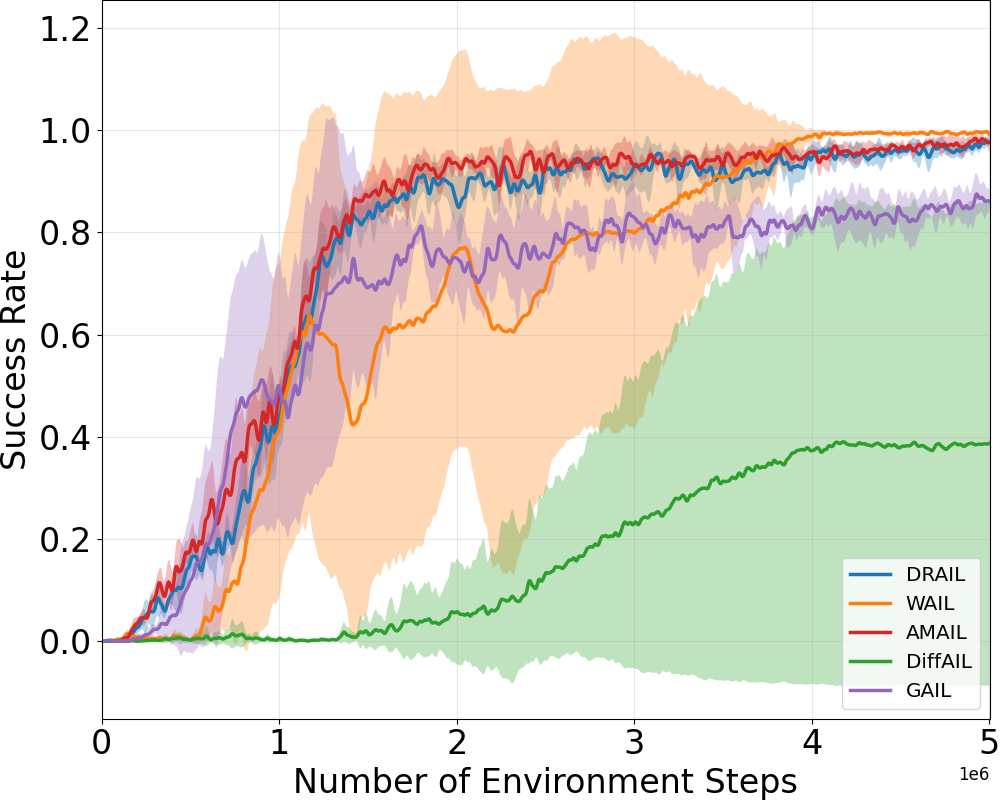
\includegraphics[width=0.33\textwidth]{2000.png}%
\label{FETCHPUSH 2000}}%


\caption{\textbf{Data efficiency}.}
\label{fig_sim3}
\end{figure*}


\begin{figure*}[!t]
\centering

\subfloat[Noise x1.25]{%
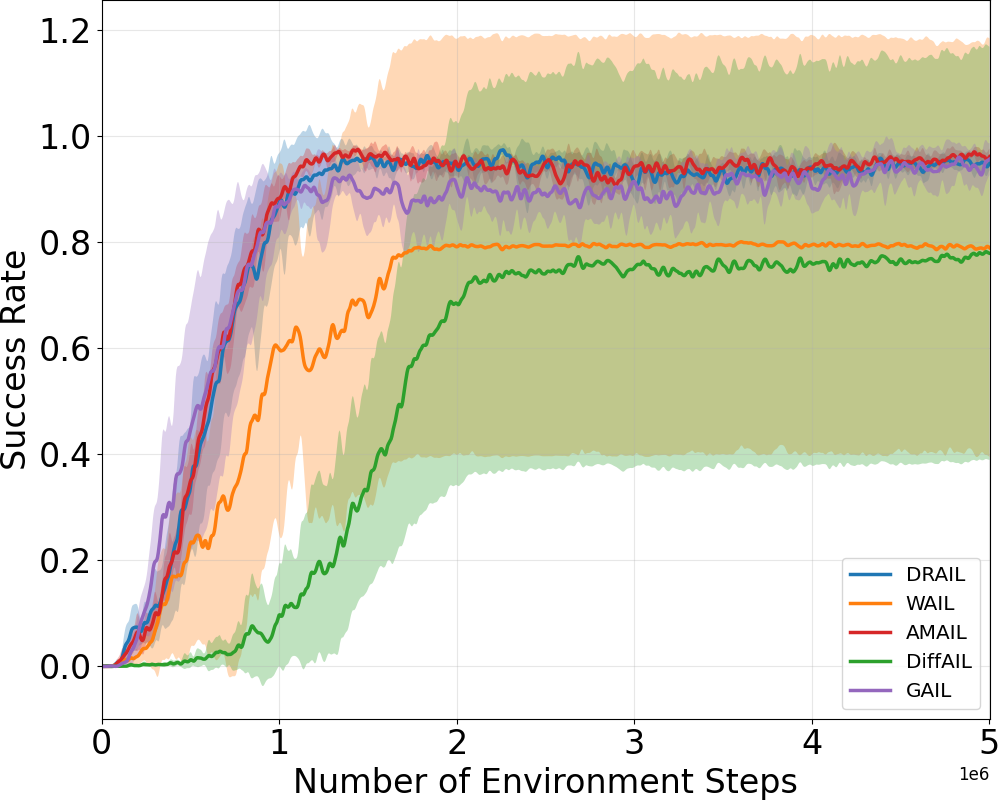
\includegraphics[width=0.33\textwidth]{1.25.png}%
\label{FETCHPUSH x1.25}}%
\hfill
\subfloat[Noise x1.75]{%
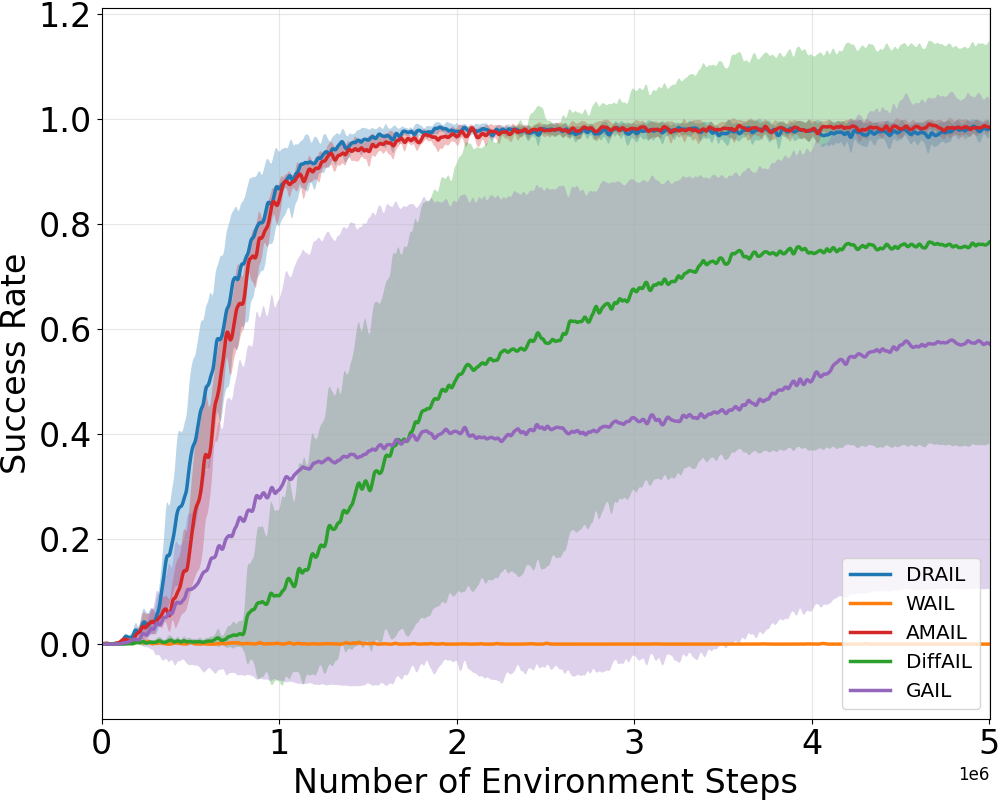
\includegraphics[width=0.33\textwidth]{1.75.png}%
\label{FETCHPUSH x1.75}}%
\hfill
\subfloat[Noise x2.00]{%
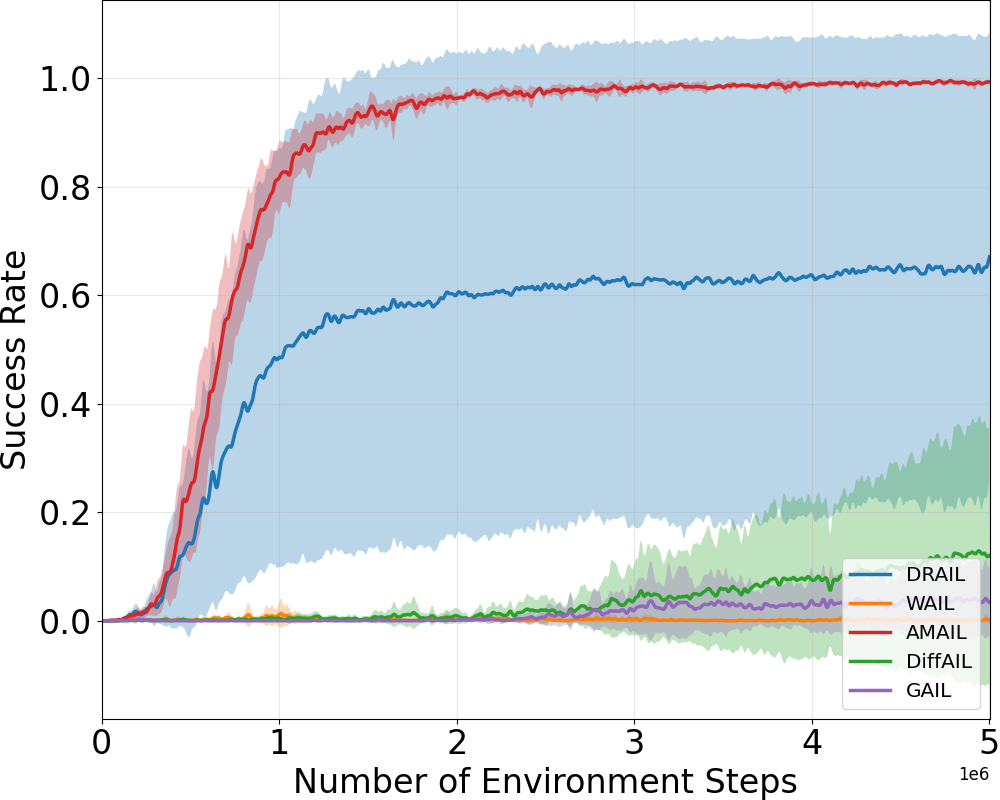
\includegraphics[width=0.33\textwidth]{2.00.png}%
\label{FETCHPUSH x2.00}}%


\caption{\textbf{Noise resistance and generalization ability}.}
\label{fig_sim4}
\end{figure*}



In contrast, some of the competitive methods showed a decline in performance as the model's data volume decreased, confirming the efficient data utilization of AMAIL.

To verify the improvement of the model's anti-noise ability and generalization ability brought by adaptive learning rate, we conducted experiments under the complete FETCHPUSH dataset with noise intensities of 1.25x, 1.75x, and 2.0x. We observed how each model performed when the noise increased and the expert data became blurred during the training process. In the experiment, noise was superimposed on the initial state and target state of the data, forcing each model to search for effective expert information in the indistinguishable state space. As shown in the figure, as the noise level increased, the traditional models experienced a significant performance collapse. The diffusion models DRAIL and DiffAIL had a higher tolerance to noise, but due to the lack of expert data, they also experienced slower training speed and performance collapse. However, AMAIL had almost no impact on the training speed and performance as the noise level increased, reflecting that the expert confidence in AMAIL can effectively suppress the systematic bias of the meta-learning network in high-noise conditions.



\section{Conclusion}
This work proposes Adaptive-Meta Generative Adversarial Imitation Learning (AMAIL), a novel framework designed to enhance imitation learning by integrating a meta-learning architecture with a diffusion-based discriminator, effectively addressing challenges of low data efficiency and noise sensitivity. We developed an adaptive meta-learning network that learns the intrinsic optimization logic from expert trajectories, enabling rapid policy adaptation. Building on this, an adaptive weighting mechanism leverages the diffusion loss to dynamically control the meta-learning's influence, ensuring robustness against suboptimal data and environmental noise. Extensive experiments on MuJoCo and PyBullet robotic control tasks demonstrate that AMAIL consistently achieves superior learning efficiency and stability, outperforming state-of-the-art methods, especially under conditions of limited data and significant noise.

Despite these results, our framework currently relies on low-dimensional state inputs. Future investigations could thus explore integrating our method with large-scale models to process high-dimensional visual data. This could also involve applying AMAIL's data-efficient learning to fine-tune pre-trained foundation policies for specialized downstream tasks, potentially accelerating their real-world deployment.


\begin{thebibliography}{1}
\bibliographystyle{IEEEtran}

\bibitem{ref1}
{\it{Mathematics Into Type}}. American Mathematical Society. [Online]. Available: https://www.ams.org/arc/styleguide/mit-2.pdf

\bibitem{ref2}
T. W. Chaundy, P. R. Barrett and C. Batey, {\it{The Printing of Mathematics}}. London, U.K., Oxford Univ. Press, 1954.

\bibitem{ref3}
F. Mittelbach and M. Goossens, {\it{The \LaTeX Companion}}, 2nd ed. Boston, MA, USA: Pearson, 2004.

\bibitem{ref4}
G. Gr\"atzer, {\it{More Math Into LaTeX}}, New York, NY, USA: Springer, 2007.

\bibitem{ref5}M. Letourneau and J. W. Sharp, {\it{AMS-StyleGuide-online.pdf,}} American Mathematical Society, Providence, RI, USA, [Online]. Available: http://www.ams.org/arc/styleguide/index.html

\bibitem{ref6}
H. Sira-Ramirez, ``On the sliding mode control of nonlinear systems,'' \textit{Syst. Control Lett.}, vol. 19, pp. 303--312, 1992.

\bibitem{ref7}
A. Levant, ``Exact differentiation of signals with unbounded higher derivatives,''  in \textit{Proc. 45th IEEE Conf. Decis.
Control}, San Diego, CA, USA, 2006, pp. 5585--5590. DOI: 10.1109/CDC.2006.377165.

\bibitem{ref8}
M. Fliess, C. Join, and H. Sira-Ramirez, ``Non-linear estimation is easy,'' \textit{Int. J. Model., Ident. Control}, vol. 4, no. 1, pp. 12--27, 2008.

\bibitem{ref9}
R. Ortega, A. Astolfi, G. Bastin, and H. Rodriguez, ``Stabilization of food-chain systems using a port-controlled Hamiltonian description,'' in \textit{Proc. Amer. Control Conf.}, Chicago, IL, USA,
2000, pp. 2245--2249.

\end{thebibliography}


\newpage

% \section{Biography Section}
% If you have an EPS/PDF photo (graphicx package needed), extra braces are
%  needed around the contents of the optional argument to biography to prevent
%  the LaTeX parser from getting confused when it sees the complicated
%  $\backslash${\tt{includegraphics}} command within an optional argument. (You can create
%  your own custom macro containing the $\backslash${\tt{includegraphics}} command to make things
%  simpler here.)
 
% \vspace{11pt}

% \bf{If you include a photo:}\vspace{-33pt}
% \begin{IEEEbiography}[{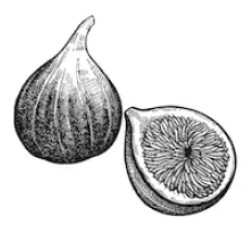
\includegraphics[width=1in,height=1.25in,clip,keepaspectratio]{fig1}}]{Michael Shell}
% Use $\backslash${\tt{begin\{IEEEbiography\}}} and then for the 1st argument use $\backslash${\tt{includegraphics}} to declare and link the author photo.
% Use the author name as the 3rd argument followed by the biography text.
% \end{IEEEbiography}

% \vspace{11pt}

% \bf{If you will not include a photo:}\vspace{-33pt}
% \begin{IEEEbiographynophoto}{John Doe}
% Use $\backslash${\tt{begin\{IEEEbiographynophoto\}}} and the author name as the argument followed by the biography text.
% \end{IEEEbiographynophoto}




\vfill

\end{document}


